\documentclass[english,11pt]{book}

% Packages
\usepackage{times}
\usepackage[T1]{fontenc}
\usepackage[utf8]{inputenc}
\usepackage{longtable}
\usepackage{float}
\usepackage{setspace}
\usepackage{verbatim}
\usepackage{textcomp}
\usepackage{amsmath}
\usepackage{units}
\usepackage{framed}
\usepackage{color}
\usepackage{enumerate}
\usepackage{babel}
\usepackage{fancyhdr}
\usepackage{fancyvrb}
\usepackage{paralist}
\usepackage{url}
\usepackage{graphicx}
\usepackage{caption}
\usepackage{subcaption}


\usepackage{xcolor}
\usepackage{showexpl}% already includes listings package
% The listings package defines an internal command for replacements within filenames. 
% One of these replacements replaces - with \textendash. 
% You can redefine this command to make the hyphens actual hyphens:
\makeatletter
\def\lst@filenamerpl{_\textunderscore $\textdollar}
\makeatother
\lstset{frame=shadowbox, basicstyle=\footnotesize\ttfamily, showstringspaces=false,
rulesepcolor=\color{black}, upquote=true}
% \lstset{language=bash, frame=shadowbox, basicstyle=\footnotesize, showstringspaces=false,
% rulesepcolor=\color{black}, upquote=true, }
\lstdefinestyle{scriptStyle}{
    basicstyle=\footnotesize,% control font of code
    preset=\footnotesize,% adjust font size of output
    numbers=left, numberstyle=\tiny, stepnumber=1, numbersep=5pt,
    frame=tlbr,
    pos=r,% want output on right
%     backgroundcolor=\color{yellow!30},
    width=0.50\linewidth,
}
\lstdefinestyle{verb}{
    basicstyle=\footnotesize,% control font of code
    preset=\footnotesize,% adjust font size of output
    frame=tlbr,
    pos=r,% want output on right
%     backgroundcolor=\color{yellow!30},
    width=0.50\linewidth,
}

\definecolor{gray}{rgb}{0.4,0.4,0.4}
\definecolor{darkblue}{rgb}{0.0,0.0,0.6}
\definecolor{cyan}{rgb}{0.0,0.6,0.6}
\lstdefinestyle{vnuml}{
    language=XML,
    basicstyle=\footnotesize,% control font of code
    preset=\footnotesize,% adjust font size of output
    frame=tlbr,
    pos=r,% want output on right
%   backgroundcolor=\color{yellow!30},
   width=0.50\linewidth,
     columns=fullflexible,
  showstringspaces=false,
  commentstyle=\color{gray}\upshape,
  stringstyle=\color{black},
  keywordstyle=\color{darkblue},
  %keywordstyle=\color{cyan},
  morekeywords={vnuml,if,vm,version,simulation_name,global,automac,vm_mgmt,vm_defaults,
  filesystem,kernel,console,net,ipv4,route,forwarding,exec,filetree,basedir,
  shell,mem,ipv6,host,ssh_version,ssh_key,netconfig,tun_device,mng_if,xterm,user},
  emph={type,id,name,mode,mask,seq,exec_mode,root},
  emphstyle=\color{cyan}
   }

%%%%%%%%%%%%%%%%%%%%%%%%%
% BEGIN Javascript!!!!! %
%%%%%%%%%%%%%%%%%%%%%%%%%
\definecolor{editorGray}{rgb}{0.95, 0.95, 0.95}
\definecolor{editorOcher}{rgb}{1, 0.5, 0} % #FF7F00 -> rgb(239, 169, 0)
\definecolor{editorGreen}{rgb}{0, 0.5, 0} % #007C00 -> rgb(0, 124, 0)
\usepackage{upquote}

\lstdefinelanguage{JavaScript}{
  morekeywords={typeof, new, true, false, catch, function, return, null, catch, switch, var, if, in, while, do, else, case, break},
  morecomment=[s]{/*}{*/},
  morecomment=[l]//,
  morestring=[b]",
  morestring=[b]'
}

\lstdefinelanguage{HTML5}{
        language=html,
        sensitive=true, 
        alsoletter={<>=-},
        otherkeywords={
        % HTML tags
        <html>, <head>, <title>, </title>, <meta, />, </head>, <body>,
        <canvas, \/canvas>, <script>, </script>,<script,!>,<p>,</p>, </body>, </html>,<html,!>, <!, html>, <style>, </style>, ><
        },  
        ndkeywords={
        % General
        =,
        % HTML attributes
        charset=, id=, width=, height=,
        % CSS properties
        border:, transform:, -moz-transform:, transition-duration:, transition-property:, transition-timing-function:
        },  
        morecomment=[s]{<!--}{-->},
        tag=[s]
}


\lstdefinestyle{Javascript}{
    % Basic design
    backgroundcolor=\color{editorGray},
    basicstyle={\scriptsize\ttfamily},   
    frame=l,
    % Line numbers
    xleftmargin={0.75cm},
    numbers=left,
    stepnumber=1,
    firstnumber=1,
    numberfirstline=true,
    % Code design   
    keywordstyle=\color{blue}\bfseries,
    commentstyle=\color{darkgray}\ttfamily,
    ndkeywordstyle=\color{editorGreen}\bfseries,
    stringstyle=\color{editorOcher},
    % Code
    language=HTML5,
    alsolanguage=JavaScript,
    alsodigit={.:;},
    tabsize=2,
    showtabs=false,
    showspaces=false,
    showstringspaces=false,
    extendedchars=true,
    breaklines=true,        
    % Support for German umlauts
    literate=%
    {Ö}{{\"O}}1
    {Ä}{{\"A}}1
    {Ü}{{\"U}}1
    {ß}{{\ss}}1
    {ü}{{\"u}}1
    {ä}{{\"a}}1
    {ö}{{\"o}}1
}

\lstdefinestyle{JavascriptTiny}{
    % Basic design
    backgroundcolor=\color{editorGray},
    basicstyle={\tiny\ttfamily},   
    frame=l,
    % Line numbers
    xleftmargin={0.75cm},
    numbers=left,
    stepnumber=1,
    firstnumber=1,
    numberfirstline=true,
    % Code design   
    keywordstyle=\color{blue}\bfseries,
    commentstyle=\color{darkgray}\ttfamily,
    ndkeywordstyle=\color{editorGreen}\bfseries,
    stringstyle=\color{editorOcher},
    % Code
    language=HTML5,
    alsolanguage=JavaScript,
    alsodigit={.:;},
    tabsize=2,
    showtabs=false,
    showspaces=false,
    showstringspaces=false,
    extendedchars=true,
    breaklines=true,        
    % Support for German umlauts
    literate=%
    {Ö}{{\"O}}1
    {Ä}{{\"A}}1
    {Ü}{{\"U}}1
    {ß}{{\ss}}1
    {ü}{{\"u}}1
    {ä}{{\"a}}1
    {ö}{{\"o}}1
}

%%%%%%%%%%%%%%%%%%%%%%%%%%%%
% END: For javascript!!!!! %
%%%%%%%%%%%%%%%%%%%%%%%%%%%%
 
   
   
   
   
\usepackage{float}
\floatstyle{plain} % optionally change the style of the new float
\newfloat{Code}{H}{myc}[chapter]
\pdfminorversion=8
%Labtel2/UPC style
% \usepackage{labtel2}
% \usepackage{UPC}
% \addto\captionsspanish{
% \renewcommand\chaptername{Practica}
% \setlength{\parindent}{0pt} }

%Exercise package
\usepackage[answerdelayed]{exercise}
\renewcommand{\ExerciseHeader}{\raggedright{\textbf{\ExerciseName\ExerciseHeaderNB
-- \ExerciseHeaderTitle\ExerciseHeaderOrigin}}}
\renewcommand{\AnswerHeader}{\medskip{\textbf{\ExerciseName\
\ExerciseHeaderNB}\smallskip}\\}
\renewcommand{\ExerciseName}{Exercise}
% Number exercises with chapter numbers.
\renewcounter{Exercise}[chapter]% Reset counter every chapter
\renewcommand{\theExercise}{~\thechapter.\arabic{Exercise}}%

%Shadowbox environment for notes JAD
\newenvironment{shadowbox}[1]%
  {
  ~\\[-0.5in]%
  \setlength\fboxsep{4pt}%
  \definecolor{shadecolor}{rgb}{0.8,0.8,0.8}%
  \begin{shaded}%
  \addtolength{\hsize}{-0.10\columnwidth}%
  {#1\\}
  }
  {
  \end{shaded}%
  \par
  }
%End Shadowbox environment for notes

%Directory definitions for .tex inputs
\newcommand{\definedir}[2]{\newcommand{#1}{#2}}
\definedir{\webrtcdir}{..}

% Version control command
\newcommand{\version}[2]{{\raggedright\textit{#1} -- versión #2}\\}

%Front cover page
\AtBeginDocument{
  \def\labelitemiii{\normalfont\bfseries{--}}
}
\makeatletter
\def\thickhrulefill{\leavevmode \leaders \hrule height 1pt\hfill \kern \z@}
\def\textoA#1{\def\@textoA{#1}}
\def\textoB#1{\def\@textoB{#1}}
\def\maketitle{%
  \null
  \thispagestyle{empty}%
  {\large \raggedleft \@textoA\par}
  \vfill
  \begin{center}\leavevmode
    \normalfont
    {\LARGE\raggedleft \@author\par}%
    \thickhrulefill\par
    {\huge\raggedright \@title\par}%
    \vskip 1cm
  \end{center}%
  \vfill
  {\large \@textoB\par}
  \null

\clearpage
  }
\makeatother
\textoA {Alex Albas\\ Gerard Auguets}
\textoB {}
\author{UPC Telematics Department}
\title{WebRTC}
%\title{Internet Protocol}
\date{}
%End of Front cover page

% Definitions of includes with if
\newif\ifPROF
\newif\ifEXTRA
\newif\ifEXTRAEXTRA
\newif\ifSOLS
% \PROFtrue
% \EXTRAtrue
% \EXTRAEXTRAtrue
% \SOLStrue
    
\begin{document}
\maketitle
\pagestyle{empty}

%\input{svn_version.tex}

\setcounter{tocdepth}{2}
\addtocontents{toc}{\protect\thispagestyle{empty}}
\tableofcontents

\pagestyle{plain}
\chapter{WebRTC\label{chap:webRTC}}
\section{Project Introduction} 

Initially we though to do our projects separately, but at the moment to choose a project related with WebRTC for Chrome\cite{Chrome}, (Generally on Firefox\cite{Mozilla}.  should work too), we realized
that the core aplication was the same, so we decided make it together and develop it with the approval of our project tutor Jose Luis.

The application that is going to be developed is web-oriented and focused on real time communications created by Google,
thing that make easier the use because no plugins and extensions are required.

To use WebRTC applications, there is not technical knowledges required so in order to use/enjoy it,only open a browser and write an URL.

To start, we did a first research in order to know what we found. After this researching, we saw for the developing of this web application
we will have to treat many aspects, which we don't have any (or a little bit) knowledge:

\begin {compactitem}
 \item WebRTC API's.\cite{webrtc,book2,book1}
 \item HTML language \cite{W3School}.
 \item JavaScript language \cite{W3School,stackoverflow}.
 \item Callback concept\cite{W3School,Socket}.
 \item Node.js Server for real time applications.\cite{Nodejs,Expressjs}
 \item Signaling process.\cite{webrtc}.
 \item Latex.
\end {compactitem}


And other knowledges related, those that have been acquired during this years at the university, thing that will make easier all the absorption of concepts above:

\begin {compactitem}
 \item Object oriented programming.
 \item Audiovisual coding.
 \item Audio/video concepts.
 \item Telematics concepts.
 \item Unix/linux environment.
\end {compactitem}


Learning all this themes suposed to us a really big challenge, due to this aplication is going to be developed from scratch, and both
(for better or worse) we have already working full time.

Once already known all the themes to treat, we began with the researching process by searching Projects, web tutorials, books, PDF, etc...spending lot of time on it
but necessary in order to be able to develop such application.

After long time researching, it was time to design our architecture application, that it was absolutely designed by us and with the approval of our tutor.
Once the architecture was created, it was time to create!

WebRTC is the present-future technology for real time communications 
and its use is greatly increasing lastly.

%FIXME BIB
%Test de Bibliography \cite{passervice,rfc4001}.


The goal of this project is to get us started with WebRTC by researching 
and understanding this technology and finally trying to develop a simple WebRTC site.
\subsection{Acknowledgments}
\begin{compactitem}
 
\item Alex:

\textbf{Nobody said it was easy but it was worth it after all}
I have to say thanks, on the one hand to Aloha and my family. My girlfriend Aloha, who has been supporting me during the lasts years staying at the university, and especially the last year. You are my engine, I love you !
Many thanks to my Parents and sister too, without them anything would have been possible.
On the other hand, to our tutor Jose Luis, who has been really involved to make it a success. Thanks Jose!
And last but not least to my university colleague and friend Gerard. We got it.

\item Gerard:

First I want to say thank to my mother for her support and unconditional love, for being with me, whenever I needed, without her I would never have achieved.
Many thanks to my father and brothers, for pushing me and motivate me to no stop never.
Finally I want to say thanks to my friends, they were always with me the few hours I could spend.
And of course, a lot of thanks to my friend Alex, thanks four your patience and energy. We got it.

\end{compactitem}
\subsection{Motivation and Objectives}
Video conferences, video-games, calls, social networks, every day the society shows clear signs of technological advance, 
allowing us to establish connections and communications with anyone, anytime, anywhere.
The exponential growth of connected devices and the access facilities to the network are the key of this
continued expansion and as in any evolving market, new technologies appear in order to improve the 
actual communication systems.
As in any engineering field, this improvements seek to improve the functional capabilities and reduce the operating cost of the systems.
The scope of this project includes all the above  with the need of establish communications in real time, approaching this practice
closer to the reality.
The main objective is to develop a web application through an expanding technology as WebRTC, that allow exchange and establish an interactive
communication and with the possibility of transferring any kind of data between two clients, in a direct way without intermediate servers and
ensuring the security and the velocity of the communication.
The application will be academic-oriented ,allowing communications between students and teachers, useful for resolving issues in real time, without
the need to travel or leave home. 
One of the main advantages is that the application doesn't require to install any plug-in or software, 
because WebRTC is implemented inside Web-Browsers. 
This facilitates the communication because both the student and the teacher can realize the communication from any computer, 
anyplace, without the need to modify the machine, only
a compatible browser is needed.

Nowadays, perhaps somebody would like to try using this technology to communicate with another person. It
can be done by visiting many demo sites such as:
\textbf{http://apprtc.appspot.com} which will create a unique URL for your video chat. Just send this URL to another
person with a browser that also supports WebRTC, and once they open that page,
users should see two video elements displayed on the page: one from your local
video camera and one from the other person's video camera. There's a lot of complex
negotiation that's gone on in the background, but assuming that Chrome/Firefox browsers are used where 
WebRTC is fully supported, thats an easy way to getting started.

In this project the following objectives have been defined taking into account the introduction themes to treat, so it was decided that the application had at least:
\begin{enumerate}
 \item A Node.js server made to manage the signaling process and text chat rooms managed by Socket.io and Express node.js  modules  node as explained in the section \ref{sec: WebRTC: Node Server}.
 \item Web design and implementation made with HTML and JavaScript languages.
 \item Be able to make a video call in a local environment and in a real environment correctly. With local environment we mean that the two browsers are on the same network and there is no Stun/Turn servers, and real environment we mean that browsers are on different networks and data go through Google Stun/turn servers.
 \item Management of video stream (pause) and audio streams (mute).
 \item Using HTTPS for a secure connection. Creating certificates to establish a secure connection, because Google Chrome only allows passage of streams if they come from this type of connection.
 \item File sharing with RTCDataChannel.

\end{enumerate}

So, with the objectives clearly defined, let's start to develop our application.

\clearpage

\section{About WebRTC}
\subsection{History}
When the World Wide Web (WWW) was first created in the early 1990's, it was built
upon a page-centric model that used HREF-based hyper-links. In this early model
of the web, browsers navigated from one page to another in order to present new
content and to update their HTML-based user interfaces.

Around the year 2000, a new approach to web browsing had started to develop, and
by the middle of that decade, it had become standardized as the XMLHttpRequest
(XHR) API. This new XHR API enabled web developers to create web applications
that didn't need to navigate to a new page to update their content or user interface. It
allowed them to utilize server-based web services that provided access to structured
data and snippets of pages or other content. This led to a whole new approach to the
web, which is now commonly referred to as Web 2.0. 

The introduction of this new XHR API enabled services such as Gmail, Facebook, Twitter, and more to create a
much more dynamic and social web for us.

Now the web is undergoing yet another transformation that enables individual web
browsers to stream data directly to each other without the need for sending it via
intermediary servers. This new form of peer-to-peer communication is built upon
a new set of API that is being standardized by the Web Real-Time Communications
Working Group available at \textbf {http://www.w3.org/2011/04/webrtc/} of the World
Wide Web Consortium (W3C), and a set of protocols standardized by Real-Time
Communication in WEB-browsers Working Group available at \textbf {http://tools.ietf.
org/wg/rtcweb/} of the Internet Engineering Task Force (IETF).
Just as the introduction of the XHR API led to the Web 2.0 revolution, the
introduction of the new WebRTC standards is creating a new revolution too.

\subsection{Introduction to Real Time Communications}
Direct peer-to-peer connections often provide lower latency, making gaming,
video streaming, sensor data feeds, and so on, appear faster and more interactive
or real-time, hence the use of this term.

Secure peer-to-peer connections allow the fact of exchanging information privately
without it being logged or managed by intermediary servers. This reduces the
need for some large service providers while creating opportunities for people to
create new types of services and applications. It introduces improved privacy for
some individuals while it may also create new complexities for regulators and law
enforcement organizations.

And the efficient peer-to-peer exchange of binary data streams removes the need to
serialize, re-encode, or convert this data at each step in the process. This leads to a
much more efficient use of network and application resources, as well as creating a
less error prone and more robust data exchange pipeline.

This is just a brief overview of how  WebRTC can be used.

%\subsection{WebRTC Introduction}
\subsection{Advantages and Drawbacks of Using WebRTC}
\subsubsection{Advantages:}

\begin{compactitem}
\item No plugins are required, just update your browser.
\item Handshaking process between the server and the participants. 
After the signaling process has been completed, the webRTC connection has been established, 
the connection is completely P2P (peer to peer).
\item Really interesting for file sharing or text chat, because the connections is being performed between the peers directly.
\item Once the connection has been established (for audio and video) the server get out of the loop 
of the connection.
\item Better encryption: The traffic is encrypted between peers, so it means that if you are being attacked 
by a MiD (man in the middle) it's really harder to break it down.
\end{compactitem}

\subsubsection{Drawbacks:}

\begin{compactitem}
\item One must be careful to not to use passwords or shared secrets at the signaling process 
because at this step data is not encrypted.
\item Not supported for all browsers: IE \& Safari are not supported.
\item Mobiles are not supported yet. No native mobile support.
\item Scaling can be hard. Large video calls are not well scaled. 
It means that if you want to do a multi chat connection, each user has to have a peer to 
peer connection with all the other users.
Right figures are 4 to 8 users. 
\end{compactitem}

\subsection{Applications and Use Cases}
The real-time web allow us to set up dynamic connections to other web browsers and web enabled devices quickly and easily.
This kind of connections open the door to a whole new range of peer-to-peer communications like:
\begin{compactitem}
\item Video conferencing.
\item Contact Centers. 
\item In-line customer support. Directly embedded into your website. 
The most simplest will be the text chat between customer and 
the support team but a call me button will be better.
\item Tele-medicine like Phemium.
\item Insurance claims. Live video feedback to your insurance company instead of calling, 
so they can see the conditions of the accident, damage of your car and so on.
\item In context communications, like company meetings, teacher-student meetings, etc.
\item Gaming, multi-player.
\item Peer file, Screen sharing, data sharing. 
\end{compactitem}
So they are very extensive its utilities.

\subsection{Supported Browsers}

Communications and Internet form a very powerful business, this can be an 
advantage to improve the technology thanks to the rivalry of companies to
take the control of the market.
On the other hand this can be a weak point too limiting the compatibility 
between the technologies developed by different manufacturers, webRTC suffer these consequences.
Fortunately the big potential of this upcoming technology is making 
companies to stop the war between them in order to take benefit of all the advantages previously commented.


\begin{figure}[htb]
\begin{centering}
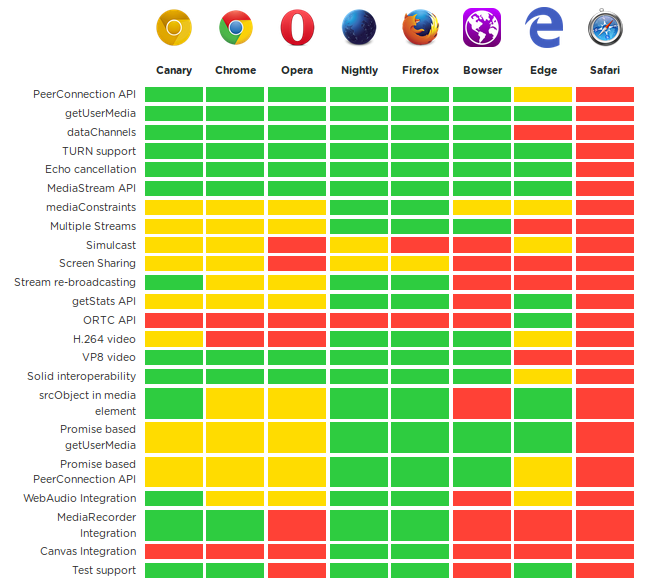
\includegraphics[width=0.7\textwidth]{\webrtcdir/figures/figuras_utilizadas/webrtc_browsers_state1.png}
\par\end{centering}
\caption{\label{fig:webrtc:supported_browsers:webrtc_browsers_state1} Browsers supported.}
\end{figure}

\section{Signaling}
\subsection{Signaling Overview}
This is a analog process like the early days of telephone. When you wanted to call somebody, the signal is picked up by telephone operator, 
which used to patch the signal with the final user. It was like a \textbf{Manual Handshake} between two parties.

Signaling \cite{HTML5rocks} is an extremely important part of webRTC. In order for a WebRTC application to set up a 'call', its clients need to exchange information:
\begin{compactitem}
\item Session control messages used to open or close communication.
\item Error messages.
\item Media meta data such as codecs and codec settings, bandwidth and media types.
\item Key data, used to establish secure connections.
\item Network data, such as a host's IP address and port as seen by the outside world.

\end{compactitem}
To avoid redundancy and to maximize compatibility with established technologies, signaling methods and protocols are not specified by WebRTC standards. 
This approach is outlined by JSEP, the \textbf{JavaScript Session Establishment Protocol}, and for this that's why signaling is not defined on WebRTC.
\clearpage
\begin{figure}[htb]
\begin{centering}
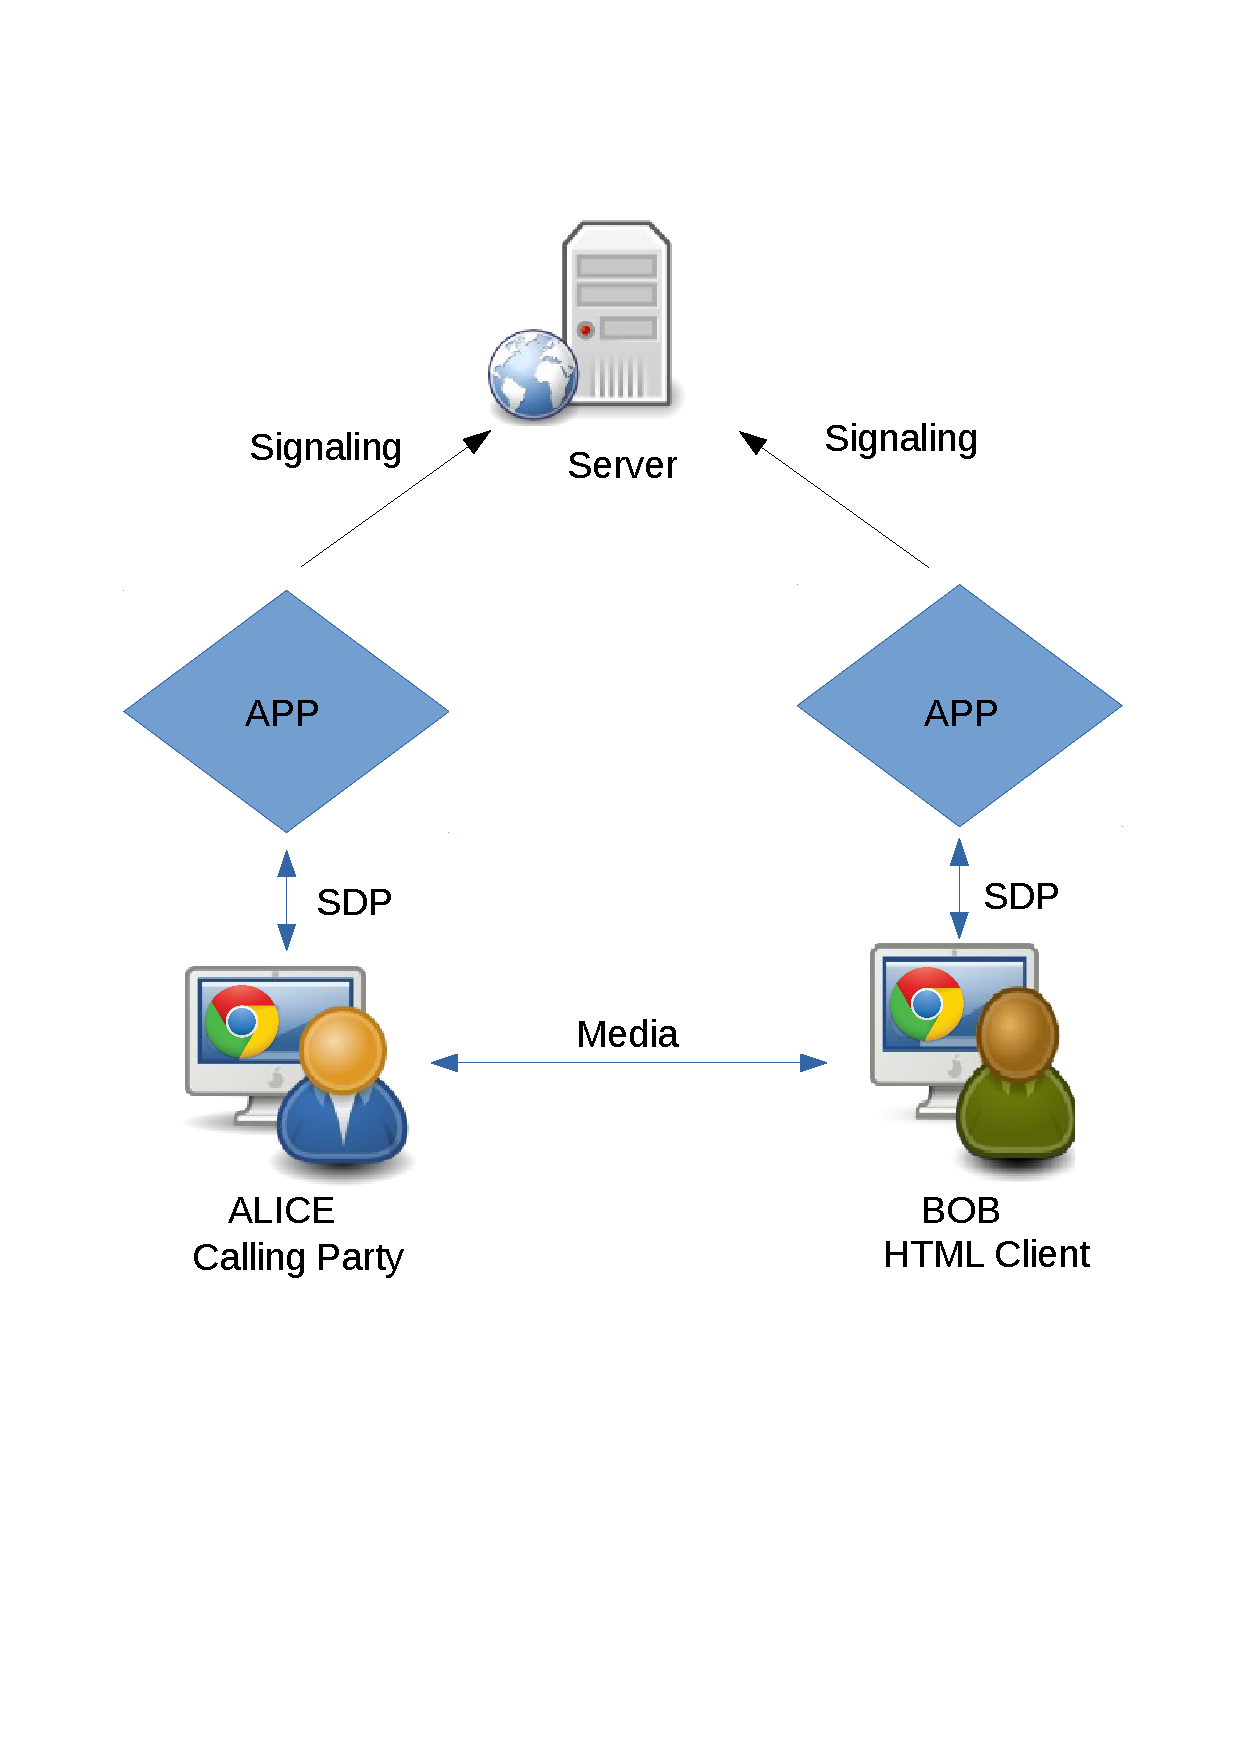
\includegraphics[width=0.6\textwidth]{\webrtcdir/figures/figuras_ok/JSEP.pdf}
\par\end{centering}
\caption{\label{fig:webrtc:SignalingOverview:JSEP}JSEP diagram}
\end{figure}
JSEP's architecture also avoids a browser having to save state: that is, to function as a signaling state machine. This would be problematic if, for example, 
signaling data was lost each time a page was reloaded. Instead, signaling state can be saved on a server.
Finally, signaling is used to set up the peer connection, which is handled by the webRTC standard by the API RTCPeerConnection which will be discussed on section \ref{sec:webrtc:WebRTC Technology} later on.
Once the RTCPeerConnection has been established, the server is not needed anymore.

The basic concepts in this kind of processes (Signaling between peers) are two:
\begin{compactitem}
\item \textbf{Offer}
\item \textbf {Answer}
\end{compactitem}
\clearpage
That's the initial scenario. Alice wants to call Bob.
%Figure \ref{fig:webrtc:SignalingOverview:4_signaling_offer_answer.pdf} Signaling offer-answer scenario
\begin{figure}[htb]
\begin{centering}
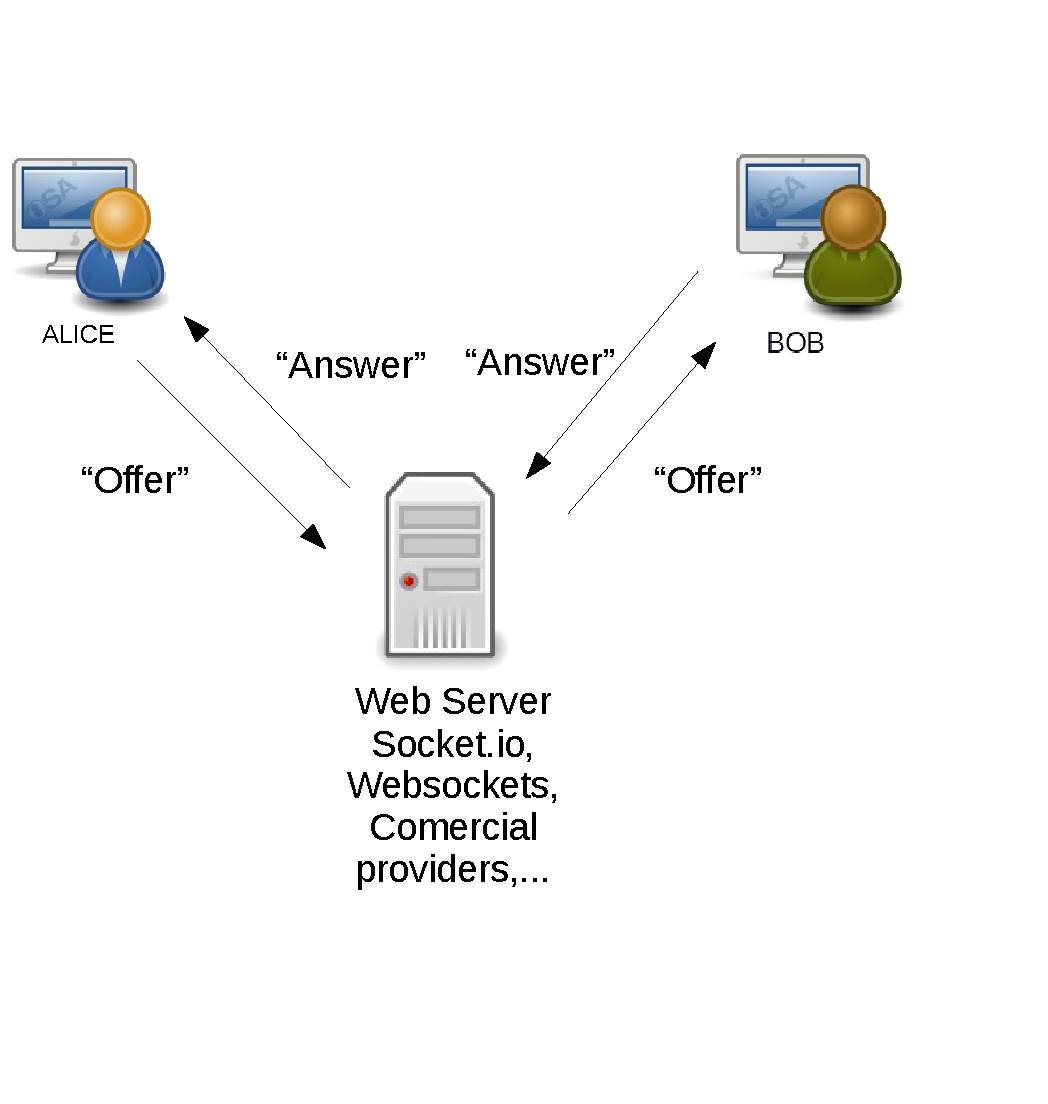
\includegraphics[width=0.7\textwidth]{\webrtcdir/figures/figuras_ok/4_signalling_offer_answer.pdf}
\par\end{centering}
\caption{\label{fig:webrtc:SignalingOverview:4_signaling_offer_answer.pdf}Signaling offer-answer scenario}
\end{figure}

Alice wants to reach Bob's browser, so an \textbf{Offer} is created to the Server.
This offer contains the Session Description Protocol\cite{rfc2327}(SDP) that features all the characteristics to the data (video \& audio) to be exchanged:
\begin{enumerate}
\item Video Codecs.
\item Resolution.
\item Format.
\item etc...
\end{enumerate}


At the same time, Bob is connected to the same server, so he receives from the server that somebody is calling him.
He clicks the button accepting the call, so he is making an \textbf{Answer}, which it will have an \textbf{Session Description Protocol (SDP)} as well.


After offer-answer model, in order to establish the Peer to Peer Connection with all the network information
is really important because on the way, information can go through Firewalls, proxy's, public Internet, etc...
So, here is when the \textbf{ICE Candidates} are starting to make sense, and they will be explained on the following section.


\clearpage
\subsection{TURN, STUN, ICE Candidates}
For meta data signaling, WebRTC API use an intermediary server, but for actual media and data streaming once a session is established, RTCPeerConnection attempts to connect clients directly: \textbf{peer to peer}.
In a simpler world, every WebRTC endpoint would have a unique address that it could exchange with other peers in order to communicate directly.
In reality most devices live behind one or more layers of NAT, some have anti-virus software that blocks certain ports and protocols, and many are behind proxies and corporate firewalls. 
A firewall and NAT may in fact be implemented by the same device, such as a home WI-FI router.

WebRTC API can use the ICE framework to overcome the complexities of real-world networking. To enable this to happen, your application must pass ICE server URL's to RTCPeerConnection.
ICE tries to find the best path to connect the Peers. 
It tries all possibilities in parallel and chooses the most efficient option that works. ICE first tries to make a connection using the host address obtained from a device's operating system and network card; if that fails (which it will for devices behind NAT's) 
ICE obtains an external address using a STUN server, and if that fails, traffic is routed via a TURN relay server.
In particular:
\begin{compactitem}
\item A STUN server is used to get an external network address.
\item TURN servers are used to relay traffic if direct (peer to peer) connection fails.
\end{compactitem}

Typically, each TURN server also supports STUN. 
That is to say, a TURN server is a STUN server with added relaying functionality built in. 
ICE also copes with the complexities of NAT setups: in reality, 
NAT 'hole punching' may require more than just a public IP: port address.
URL's for STUN and/or TURN servers are (optionally) specified by a WebRTC API 
in the iceServers configuration object that is the first argument to the RTCPeerConnection constructor. 

%Figure \ref{fig:webrtc:SignalingOverview:4_IceServer.png} Ice Servers



\begin{lstlisting}[style=JavaScript]
{
'iceServers': [
  {
    'url': 'stun:stun.l.google.com:19382'
    },
    {
    'url': 'turn:192.158.29.39:3478?transport=udp',
    'credential': 'JZEOEt2V3Qb0y27GRntt2u2PAYA=',
    'username': '2824511:1379330808'
    },
    {
    'url': 'turn:192.158.29.39:3478?transport=tcp',
    'credential': 'JZEOEt2V3Qb0y27GRntt2u2PAYA=',
    'username': '2824511:1379330808'
    }
  ]
}
\end{lstlisting}

Once RTCPeerConnection has that information, the ICE magic happens automatically: RTCPeerConnection uses the ICE framework to work out the best path between peers, working with STUN and TURN servers as necessary.
\begin{enumerate}
 
\item \textbf{STUN Servers}:

NAT's provide a device with an IP address for use within a private local network, but this address can't be used externally. Without a public address, there's no way for WebRTC peers to communicate. 
To get around this problem WebRTC uses STUN.
STUN servers live on the public Internet and have one simple task: check the IP port address of an incoming request (from an application running behind a NAT) and 
send that address back as a response. In other words, the application uses a STUN server to discover its IP:Port from a public perspective. 
This process enables a WebRTC peer to get a publicly accessible address for itself, and then pass that on to another peer via a signaling mechanism, in order to set up a direct link. (In practice, different NAT's work in different ways, and there may be multiple NAT layers, but the principle is still the same.)
STUN servers don't have to do much or remember much, so relatively low-spec STUN servers can handle a large number of requests.
Most WebRTC calls successfully make a connection using STUN: 86\%, according to www.webrtcstats.com, though this can be less for calls between peers behind firewalls and complex NAT configurations.
%TODO image of STUN server

\item \textbf{TURN Servers}:

RTCPeerConnection tries to set up direct communication between peers over UDP. If that fails, RTCPeerConnection resorts to TCP. If that fails, 
TURN servers can be used as a fall back, relaying data between endpoints.

Just to reiterate: TURN is used to relay audio/video/data streaming between peers, not signaling data.
TURN servers have public addresses, so they can be contacted by peers even if the peers are behind firewalls or proxies. TURN servers have a conceptually simple task to relay a stream but, unlike STUN servers, 
they inherently consume a lot of bandwidth. In other words, TURN servers need to be beefier.

\end{enumerate}
WebRTC is not made for this, due to it is translated to too latency, unthinkable fact on a real time communications. So, here is when \textbf{ICE Framework} appears.

Peers must exchange information about the network connection. This is known as an \textbf{ICE Candidate} and details the available methods the peer is able to communicate (directly or through a TURN server).

\clearpage

\subsection{Signaling Diagram}
The signaling diagram explained in a figure, that's a way to try to understand what's going on in this process:

%Figure \ref{fig:webrtc:SignalingOverview:4_signaling_diagram.pdf} Signaling states
\begin{figure}[htb]
\begin{centering}
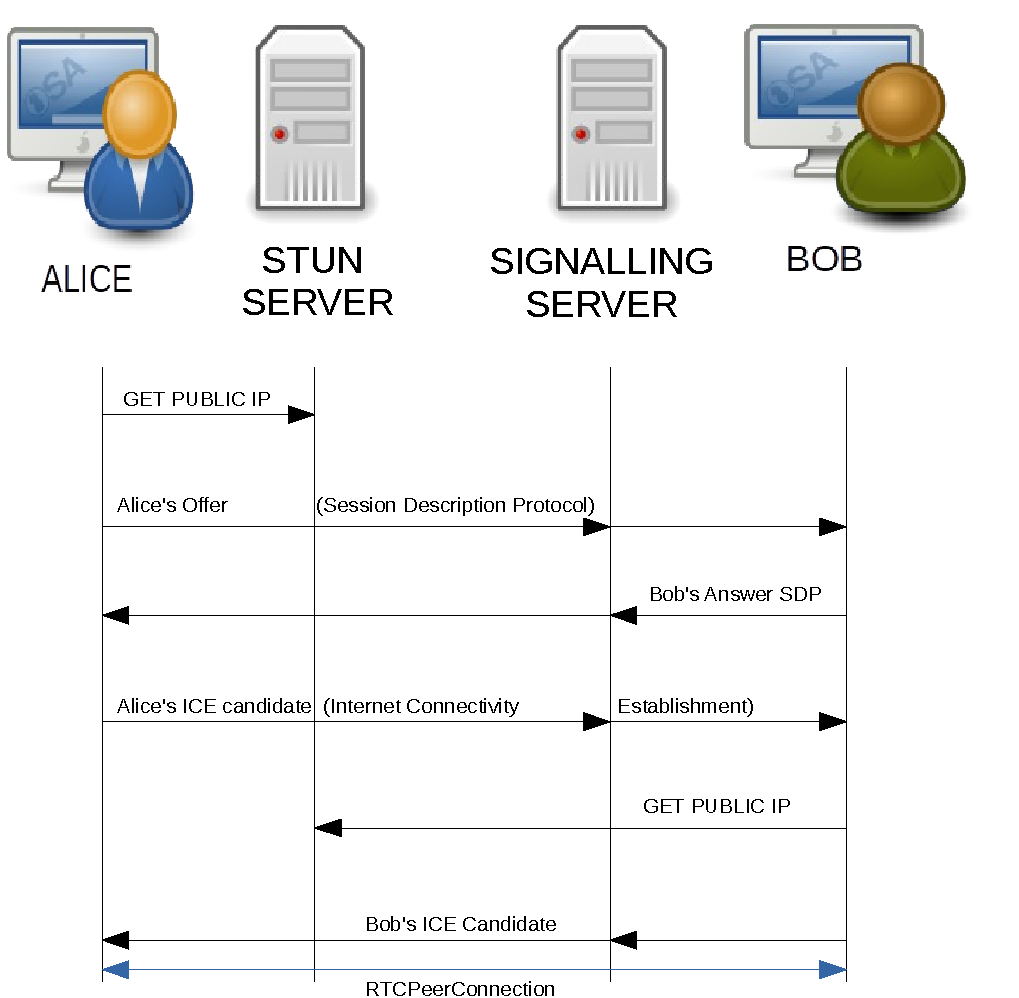
\includegraphics[width=0.7\textwidth]{\webrtcdir/figures/figuras_ok/4_signalling_diagram.pdf}
\par\end{centering}
\caption{\label{fig:webrtc:SignalingOverview:4_signaling_diagram.pdf}Signaling states}
\end{figure}

\begin{compactitem}
\item An Public IP is obtained by STUN server for Alice in order to get out to the Internet.
\item Alice sends an \textbf{Offer} to bob through the Signaling server.
\item Bob accepts it by sending an \textbf{Answer} to Alice through the Signaling Server.
\item ICE Candidate is going back and forward between Alice and Bob by the Signaling Server.
\item In this case, both could get an public IP, but if there is a firewall in the middle, other IP they will get.
\item When an ICE candidate is ready, it is possible to establish an RTCPeerConnection
\end{compactitem}
\clearpage

\subsection{Session Description Protocol (SDP) \label{sec:webrtc:sdp}}
The configuration of an endpoint on a WebRTC connection is called a session description. The description includes information about the kind of media being sent, its format, the transfer protocol being used, the endpoint's IP address and port, 
and other information needed to describe a media transfer endpoint. 
This information is exchanged and stored using Session Description Protocol \cite{WebRTCHacks} (SDP); if you want details on the format of SDP data, you can find it in RFC 2327.

When a user starts a WebRTC call to another user, a special description is created called an offer. 
This description includes all the information about the caller's proposed configuration for the call. The recipient then responds with an answer, which is a description of their end of the call. 
In this way, both devices share with one another the information needed in order to exchange media data. This exchange is handled using Interactive Connectivity Establishment (ICE, a protocol which lets two devices use an intermediary
to exchange offers and answers even if the two devices are separated by Network Address Translation (NAT).

Each peer, then, keeps two descriptions on hand: the local description, describing itself, and the remote description, describing the other end of the call.

The offer/answer process is performed both when a call is first established, but also any time the call's format or other configuration needs to change. Regardless of whether it's a new call, or reconfiguring an existing one, 
these are the basic steps which must occur to exchange the offer and answer:

\begin{compactitem}
\item Alice calls RTCPeerConnection.createOffer() to create an offer.
\item Alice calls RTCPeerConnection.setLocalDescription() to set that offer as the local description (that is, the description of the local end of the connection).
\item Alice uses the signaling server to transmit the offer to the intended receiver of the call.
\item Bob receives the offer and calls RTCPeerConnection.setRemoteDescription() to record it as the remote description (the description of the other end of the connection).
\item Bob does any setup it needs to do for its end of the call, including adding outgoing streams to the connection.
\item Bob then creates an answer by calling RTCPeerConnection.createAnswer().
\item Bob calls RTCPeerConnection.setLocalDescription() to set the answer as its local description. Bob now knows the configuration of both ends of the connection.
\item Bob uses the signaling server to send the answer to Alice.
\item Alice receives the answer.
\item Alice calls RTCPeerConnection.setRemoteDescription() to set the answer as the remote description for its end of the call. It now knows the configuration of both peers. Media begins to flow as configured.
Pending and current descriptions
\end{compactitem}
Taking one step deeper into the process, we find that localDescription and remoteDescription, the properties which return these two descriptions, aren't as simple as they look. Because during renegotiation, an offer might be rejected because it proposes an incompatible format, 
it's necessary that each endpoint have the ability to propose a new format but not actually switch to it until it's accepted by the other peer. 
For that reason, WebRTC uses pending and current descriptions.

The current description (which is returned by the RTCPeerConnection.currentLocalDescription and RTCPeerConnection.currentRemoteDescription properties) represents the description currently in actual use by the connection. 
This is the most recent connection that both sides have fully agreed to use.

The pending description (returned by RTCPeerConnection.pendingLocalDescription and RTCPeerConnection.pendingRemoteDescription) indicates a description which is currently under consideration following a call to  setLocalDescription() or setRemoteDescription(), respectively.

When reading the description (returned by RTCPeerConnection.localDescription and RTCPeerConnection.remoteDescription), the returned value is the value of pendingLocalDescription/pendingRemoteDescription if there's a pending description (that is, the pending description isn't null); otherwise, the current description (currentLocalDescription/currentRemoteDescription) is returned.

When changing the description by calling setLocalDescription() or setRemoteDescription(), the specified description is set as the pending description, and the WebRTC layer begins to evaluate whether or not it's acceptable. Once the proposed description has been agreed upon, the value of currentLocalDescription or currentRemoteDescription is changed to the pending description, 
and the pending description is set to null again, indicating that there isn't a pending description.

\subsubsection{SDP Architecture}

Below table introduces high-level breakup of SDP into components that semantically describe a multimedia session,
oriented in to a WebRTC session.

SDP Components:

\begin{compactitem}
\item Session Description
\item Time Description
\item Media Description
\end{compactitem}
An SDP session description consists of a number of lines of text of the form:
\texttt{<type>=<value>}.
where <type> must be exactly one case-significant character and <value> is structured text whose format depends on <type>.  
In general, <value> is either a number of fields delimited by a single space character or a free format string, and is case-significant
unless a specific field defines otherwise.  Whitespace must not be used on either side of the "=" sign.

Some lines in each description are required and some are optional,but all must appear in exactly the order given here (the fixed order
greatly enhances error detection and allows for a simple parser). Optional items are marked with a "*".
\clearpage
\begin{table}[h]
\caption{Session Description}
\label{tbl:MediaStreamTrack methods}
\centering
\begin{footnotesize}
\begin{tabular}{l p{10cm}}
\hline
\texttt{v=} & Protocol version\\
\texttt{o=} & Originator and session identifier\\
\texttt{s=} & Session name\\
\texttt{i=*} & Session information\\
\texttt{u=*} & URL description\\
\texttt{e=*} & E-mail address\\
\texttt{p=*} & Phone number\\
\texttt{c=*} & Connection information\\
\texttt{b=*} & Bandwidth information\\
\texttt{z=*} & Time zone adjustments\\
\texttt{k=*} & Encryption key\\
\texttt{a=*} & Attribute information\\
\hline 
\end{tabular}
\end{footnotesize}
\end{table} 
%%SEPARACION
\begin{table}[h]
\caption{Time Description}
\label{tbl:MediaStreamTrack methods}
\centering
\begin{footnotesize}
\begin{tabular}{l p{10cm}}
\hline
\texttt{t=} & Time the session is active\\
\texttt{r=*} & Repeat session times\\
\hline 
\end{tabular}
\end{footnotesize}
\end{table} 
%%SEPARACION
\begin{table}[h]
\caption{Media Description}
\label{tbl:MediaStreamTrack methods}
\centering
\begin{footnotesize}
\begin{tabular}{l p{10cm}}
\hline
\texttt{m=} & Media name and transport address\\
\hline 
\end{tabular}
\end{footnotesize}
\end{table} 
\clearpage

SDP example:
\begin{lstlisting}
v=0;
o= jdoe 2890844526 2890842807 IN IP4 10.47.16.5;
s= SDP WebRTC Alex-Gerard;
i= A example of SDP used in WebRTC;
u=http://Alex-Gerard-EetWebRTC-PFG.com;
e=j.eetwebrtc@gmail.com (Alex Albas, Gerard Auguets);
c=IN IP4 224.2.17.12/127;
t=2873397496 2873404696;
m= audio 54609 UDP/TLS/RTP/SAVPF;
a=rtpmap:0 PCMU/8000;
a=rtcp-mux; \\Alice can perform RTP/RTCP Mux
a=rtcp:54609 IN IP4 24.23.204.141 \\Port for RTCP data
a=ptime:60   \\Audio packetization of 60 ms
a=sendrecv \\Alice can send and receive audio
a=setup:actpass \\Alice can perform DTLS before answer arrives
a=fingerprint:sha-1 99:41:49:83:4a:97:0e:1f:ef:6d:f7:c9:c7:70:
9d:1f:66:79:a8:07 \\DTLS Fingerprint for SRTP
a=ice-ufrag:074c6550 \\ICE user fragment 
a=ice-pwd:a28a397a4c3f31747d1ee3 \\ICE password       
a=candidate:0 1 UDP  2122194687 
192.168.1.4 54609 typ host \\RTP Host Candidate
a=candidate:0 2 UDP 2122194687        
192.168.1.4 54609 typ host \\RTCP Host Candidate    
a=candidate:1 1 UDP  1685987071 24.23.204.141 64678 typ srflx        
addr 192.168.1.4 rport 54609  \\RTP Server Reflexive ICE Candidate 
a=candidate:1 2 UDP  1685987071 24.23.204.141 64678 typ srflx 
raddr 192.168.1.4 rport 54609\\RTCP Server Reflexive Candidate
a=rtcp-fb:109 nack \\Indicates NACK RTCP feedback support
a=rtcp-rsize Alice intends to use reduced size RTCP for this session   
\end{lstlisting}

\clearpage

\subsection{Node Server  \label{sec: WebRTC: Node Server} }
\subsubsection{About Node}
Node\cite{Nodejs} is an interface to the V8 JavaScript runtime  the super-fast JavaScript interpreter that runs in the Chrome browser. As it happens, you can also download V8 and embed it into anything; Node does that, for web servers. 
JavaScript is after all, just a language there's nothing that says it couldn't be used on a server as well as in the users browser. In a typical LAMP server stack, there is an underlying Apache or NGINX web server, with PHP running on top of it. Each new connection to the server spawns a new thread, and it's very easy to quickly lose performance or for a site to go down. 
the only way to support more users being to add more servers. It simply doesn't scale well. With Node, this isn't the case. There is no Apache to listen for incoming connections and return HTTP status codes so node will need to handle that core server architecture itself. Luckily, there is modules to make this easier, but it can still be a little overwhelming at the beginning. 
The result, however, is a high performance web application.

It is used to develop I/O intensive web applications like video streaming sites, single-page applications, and other web applications. Node.js is open source, completely free, and used by thousands of 
developers around the world.

In this project just Node.js and some specifications are introduced in order to understand the WebRTC application that has been created.

\subsubsection{Node Features}
The following features make node.js essential for any of software architects:

\begin {compactitem}
\item \textbf{Asynchronous and event Driven}: All API of Node.js library are asynchronous (Non-blocking code), so it means that the server never waits for an API to return data.
The server will move to the next API after calling it and the notification mechanism of Events of Node.js helps the server to get a response from the previous call.
\item \textbf{Really fast}: Node.js library is very fast in code execution because it is built on Google Chrome's V8 JavaScript Engine.
\item \textbf{Highly Scalable with single Threated model}: This technologies uses a single threated model with event looping which helps the server to respond in a non-blocking code and it makes
the server really scalable instead of the traditional servers that just can handle a limited number of threads.
Node.js can provide service to high number of requests than typical servers like Apache HTTP server.
\item \textbf{No storing data}: There is no data buffered, just output the data in chunks.
\item \textbf{MIT license}: https://raw.githubusercontent.com/joyent/node/v0.12.0/LICENSE
\end{compactitem}
\clearpage
\subsubsection{Main Concepts}
The following diagrams shows some of the most important concepts(there are much more of them) that node offers to anybody who wants to use it:
\begin{figure}[htb]
\begin{centering}
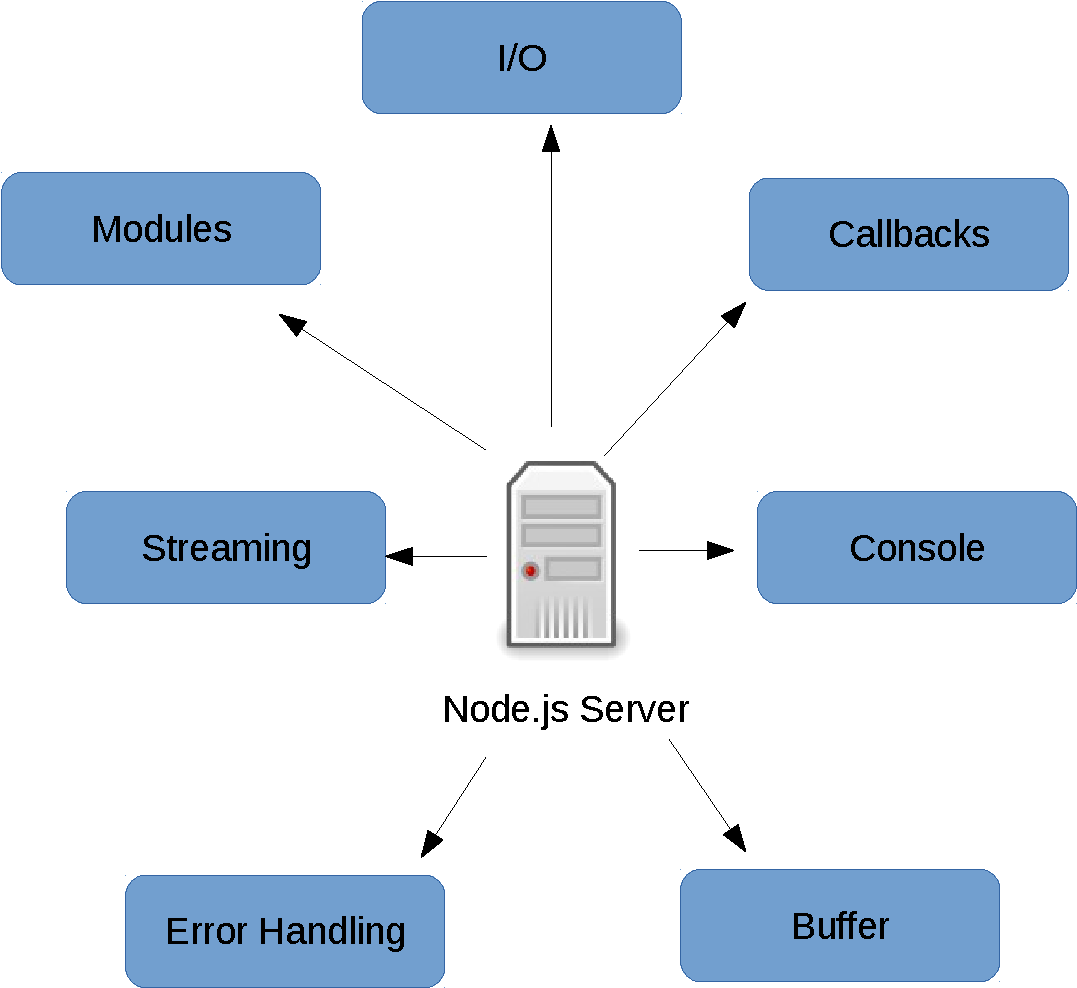
\includegraphics[width=0.7\textwidth]{\webrtcdir/figures/figuras_ok/node_MainConcepts.pdf}
\par\end{centering}
\caption{\label{fig:webrtc:SignalingOverview:node_MainConcepts.pdf}Node Main concepts}
\end{figure}

\begin {compactitem}
\item \textbf{Console \& Debugging}: The console module provides a simple debugging console that is similar to the JavaScript console mechanism provided by web browsers. The best debugger is console.log(), 
but sometimes it is needed in order to see the call stack and orient yourself in asynchronous code a bit more.
The server will move to the next API after calling it and the notification mechanism of Events of Node.js helps the server to get a response from the previous call.

The following example show how it works:
\begin{lstlisting}[style=JavaScript]

console.log('hello world');
  // Prints: hello world, to stdout
console.log('hello %s', 'world');
  // Prints: hello world, to stdout
console.error(new Error('Whoops, something bad happened'));
  // Prints: [Error: Whoops, something bad happened], to stderr

const name = 'Will Robinson';
console.warn(`Danger ${name}! Danger!`);
  // Prints: Danger Will Robinson! Danger!, to stderr

  
\end{lstlisting}
\item \textbf{Callbacks}:Callback is an asynchronous equivalent for a function. A callback function is called at the completion of a given task. Node makes heavy use of callbacks. All API of Node are written in such a way that they supports callbacks.

For example, a function to read a file may start reading file and return the control to execution environment immediately so that next instruction can be executed. Once file I/O is complete, it will call the callback function while passing the callback function, the content of the file as parameter. 
So there is no blocking or wait for File I/O. 
This makes Node.js highly scalable, as it can process high number of request without waiting for any function to return result.

Example:
\begin{lstlisting}[style=JavaScript]

fs.readdir(source, function(err, files) {
  if (err) {
    console.log('Error finding files: ' + err)
  } else {
    files.forEach(function(filename, fileIndex) {
      console.log(filename)
      gm(source + filename).size(function(err, values) {
        if (err) {
          console.log('Error identifying file size: ' + err)
        } else {
          console.log(filename + ' : ' + values)
          aspect = (values.width / values.height)
          widths.forEach(function(width, widthIndex) {
            height = Math.round(width / aspect)
            console.log('resizing ' + filename + 'to ' + height + 'x' + height)
            this.resize(width, height).write(destination + 'w' + width + '_' + filename, function(err) {
              if (err) console.log('Error writing file: ' + err)
            })
          }.bind(this))
        }
      })
    })
  }
})


  
\end{lstlisting}

\item \textbf{I/O Files}: Reading and writing from/to The files system is done by the 'fs' module. There two sets of methods: Asynchronous and Synchronous. 
For example, if a file is required to be read, it can be done by using this two modalities:
    \begin{compactitem}
    \item Asynchronous: 
    \begin{lstlisting}[style=JavaScript]
    var fs = require('fs');
    fs.readFile('/etc/passwd', function(err, buf) {
      console.log(buf.toString());
    });

    \end{lstlisting}
    Node will continue executing any JavaScript code it encounters while reading the file. 
    Once all JavaScript is done being executed and the file is ready, it will run the anonymous function and print the file contents.
    \item Synchronous:
    \begin{lstlisting}[style=JavaScript]
    var fs = require('fs');
    var contents = fs.readFileSync('/etc/passwd').toString();
    console.log(contents);
    \end{lstlisting}
    In this example, the contents variable will be set to the contents of the file, and no JavaScript code will be executed while the file is being read.

    \end{compactitem}
\clearpage
\item \textbf{Streaming}: Streaming data is a term that mean an application processes the data while it's still receiving it. 
This is useful for extra large datasets, like video or database migrations.
\begin{lstlisting}[style=JavaScript]
var fs = require('fs');
fs.createReadStream('./data/users.csv').pipe(process.stdout);
\end{lstlisting}

\item \textbf{Export Modules}:A module encapsulates related code into a single unit of code. When creating a module, this can be interpreted as moving all related functions into a file.
It can be explained with a simple example, in order to catch the main idea of what is a module:
    \begin{compactitem}
    \item Imagine this sample of code:
    \begin{lstlisting}[style=JavaScript]
    // HelloHola.js
    sayHelloInEnglish = function() {
      return "Hello";
    };

    sayHelloInSpanish = function() {
      return "Hola";
    };
 
    \end{lstlisting}
    \item \textbf{Exporting a module}:The utility of HelloHola.js increases when its encapsulated code can be utilized in other files. So let's redactor \texttt{HelloHola.js} to achieve this goal. 
    \begin{lstlisting}[style=JavaScript]
     module.exports = {
	sayHelloInEnglish: function() {
	  return "HELLO";
	},
       
	sayHelloInSpanish: function() {
	  return "Hola";
	}
    };
    \end{lstlisting}
    \item  \textbf{Importing a module}:The keyword 'require' is used in Node.js to import modules, so in this ways the previous exported modules can be used as many times as needed.
    \begin{lstlisting}[style=JavaScript]
     // main.js
     var greetings = require("./greetings.js");
     
     //-----Same as above----
     // main.js
    var greetings = {
      sayHelloInEnglish: function() {
	return "HELLO";
      },
       
      sayHelloInSpanish: function() {
	return "Hola";
      }
    };
     
    \end{lstlisting}


\end{compactitem}
\item \textbf{Buffer}: Buffer is a Node.js addition to four primitives (boolean, string, number and RegExp) and all-encompassing objects (array and functions are also objects) in front-end JavaScript. We can think of buffers as extremely efficient data stores.
In fact, Node.js will try to use buffers any time it can, e.g., reading from file system, receiving packets over the network.    
  
\end{compactitem}

\clearpage
\subsubsection{Environment Setup}
In order to make a local setup environment for Node.js, some basic steps are required:
\begin{compactitem}
\item \textbf{Text editor}, such as Notepad, Sublime text, vim , vi, etc...
\item \textbf{Install the Node.js binary}: The files  created with the text editor are called source files and contain program source code. The source files for Node.js programs are typically named with the extension ".js".
In order to install on UNIX/Linux/Mac OS X:
\begin{enumerate}
 \item Download and extract the archive node-v0.XX.\textbf{OSName}.tar.gz into /tmp.
 \item Move the extracted files into /usr/local/nodejs directory.
 
 For example: 
    \begin{lstlisting}
      $ sudo apt-get install nodejs
    \end{lstlisting}
    Add \texttt{/usr/local/nodejs/bin} to the PATH environment variable.
     \begin{lstlisting}
     $ export PATH=/usr/local/nodejs/bin
    \end{lstlisting}
    

\end{enumerate}
\item \textbf{Executing a Node.js file}:
Executing a Node file is really simple, but it will be explained with a simple web HTTP server example:
\begin{enumerate}
 \item Create a file named 'server.js' a fill with code below:

  \begin{lstlisting}[style=JavaScript]
     var http = require('http');
     http.createServer(function (req, res) {
	res.writeHead(200, {'Content-Type': 'text/plain'});
	res.end('Hello World\n');
    }).listen(1337, '127.0.0.1');
    console.log('Server running at http://127.0.0.1:1337/');]
  \end{lstlisting}
\item Open the console and execute the js file.
    \begin{lstlisting}
     $ node server.js
    \end{lstlisting}
\item As a result, it will be prompted on the console
    \begin{lstlisting}
      Server running at http://127.0.0.1:1337/
    \end{lstlisting}
\end{enumerate}
\item \textbf{NPM install};
The Node Packages Modules provides two basic functionalities:
\begin{enumerate}
 \item Access to on line repositories (packages/modules) to use them.
 \item Command line utility to install this packages and version/dependency management like apt-get on Linux.
 
\end{enumerate}
In order to install a package, exist this simple syntax:
\begin{lstlisting}
      $ npm install express
 \end{lstlisting}
 And for using them, just require command is used at the beginning on the JavaScript code:
 \begin{lstlisting}
      var express = require('express');
 \end{lstlisting}
 


\end{compactitem}

\clearpage

\subsection{Node.js Used Modules}
\subsubsection{Socket.io}
\begin{enumerate}

\item \textbf{Socket.io Overview: }

It's important to provide timely feedback to users in your web application. It all started with the introduction of XMLHttpRequest by Microsoft which became what we now know as AJAX. 
AJAX long-polling used to be the standard way to fetch server-sent data for an application, though it wasn't the most ideal solution. Long-polling involves sending periodic HTTP requests for data, introducing latency and increasing server load.

The IETF standardized Web Sockets in 2011, providing a way for developers to send and receive data through a TCP socket. All major browsers began to roll out support for the standard, and developers started to use it in their projects.

Socket.IO\cite{Socket.io} is an event-based bi-directional communication layer for real time web applications, built atop Engine.IO. It abstracts many transports, including AJAX long-polling and Web Sockets, into a single API. It allows developers to send and receive data without worrying about cross-browser compatibility.

\item \textbf{First Major Release:}

Socket.IO finally reached version 1.0 on the 28th of May, 2014. The Socket.IO project contained two parts before 1.0: a transport handling implementation, and a high-level API. Transport handling has been moved out into a separate, framework-agnostic project: Engine.IO. 
This allows other developers to build new API and projects for the real time web without reinventing the wheel.

Apart from architectural changes, Socket.IO 1.0 introduces many user-facing changes, including:
\begin{compactitem}
 \item Binary streaming support.
 \item Improved support for horizontal scaling.
 \item Removal of cluttered debug messages in the console by default.
 \item Support for Node.js streams via the socket.io-stream module.
\end{compactitem}

\item \textbf{The Basics:}
Socket.IO provides both server-side and client-side components with similar API.

\begin{compactitem}
 \item \textbf{Server-side}: On the server-side, Socket.IO works by adding event listeners to an instance of http.Server.
 \begin{lstlisting}[style=JavaScript]
var server = require("net").createServer();  
var io = require("socket.io")(server);

var handleClient = function (socket) {  
    // we've got a client connection
    socket.emit("tweet", {user: "nodesource", text: "Hello, world!"});
};

io.on("connection", handleClient);

server.listen(8080);  
 \end{lstlisting}
 \item \textbf{Client-side}: The HTTP server will begin to serve the client library at /socket.io/socket.io.js. To connect to our Socket.IO server, is needed to put the following in the body tag:
 \begin{lstlisting}[style=JavaScript]
<script src="/socket.io/socket.io.js"></script>  
<script>  
    var socket = io.connect("http://localhost");
</script>  
 \end{lstlisting}
\end{compactitem}



\end{enumerate}

\subsubsection{Express}
\begin{enumerate}
 


\item \textbf{Express Overview}:
Express \cite{Express.js} is a minimal and flexible Node.js web application framework that provides a robust set of features for web and mobile applications.
Express is a really handy Node.js module in order to handling with the common conventions when writing web applications. It includes:
\begin{compactitem}
 \item Writing API's.
 \item Handling request and responses.
 \item Routing data.
 \item Managing Front-end rendering.
\end{compactitem}
\item \textbf{Routing}:
It refers to the definition of application end points (URiS) and how they respond to client requests.
Example of a really basic route:
\begin{lstlisting}[style=JavaScript]
 var express = require('express');
var app = express();

// respond with "hello world" when a GET request is made to the homepage
app.get('/', function(req, res) {
  res.send('hello world');
});

\end{lstlisting}
\begin{compactitem}
 


\item \textbf{Typical Route methods}:
A route method is derived from one of the HTTP methods, and is attached to an instance of the express class. The following code shows two typical route methods to the root of the API:
\begin{lstlisting}[style=JavaScript]
// GET method route
app.get('/', function (req, res) {
  res.send('GET request to the homepage');
});

// POST method route
app.post('/', function (req, res) {
  res.send('POST request to the homepage');
});


\end{lstlisting}
\item \textbf{Route paths}:
In combination with a request method, define endpoints at which request can be made. Route paths can be strings, string patterns or regular expressions.
Here there are some route paths String-based examples:

This route path will match requests to the root route, '/'.
\begin{lstlisting}[style=JavaScript]
app.get('/', function (req, res) {
  res.send('root');
});

\end{lstlisting}

This route path will match requests to /about:
\begin{lstlisting}[style=JavaScript]
app.get('/about', function (req, res) {
  res.send('about');
});

\end{lstlisting}


\item \textbf{Response methods}:
The methods on the response object (res) can send a response to the client, and terminate the request-response cycle.
If none of these methods are called from a route handler, the client request will be left hanging.
Here some examples of the most common used response methods:

It will render the 'index.ejs' to the client that has made a request by including on the response.
\begin{lstlisting}[style=Javascript]
 app.get('/', function(req, res){
    res.render('index.ejs');
});
\end{lstlisting}
It will send a response of various types:
\begin{lstlisting}[style=javascript]
 router.get('/', function(req, res){
  res.send('hello world');
});
\end{lstlisting}
Prompt a file to be downloaded:
\begin{lstlisting}[style=javascript]
 router.get('/download', function(req, res){
  res.send('/res.download('/report-12345.pdf');');
});
\end{lstlisting}



\end {compactitem}


\end{enumerate}
\subsubsection{Express + Socket.io = Express.io}
The result of combining Socket.io and Express results Express.io, a real time-web framework for node.js. In this project this framework is used in order to take advantage of 
some of characteristics from this really powerful modules.
\clearpage


\section{WebRTC Technology}

\subsection{JavaScript Introduction}

JavaScript\cite{W3School}is an object-oriented dynamic language with types and operators, standard built-in objects,
and methods. 
Object-oriented languages can be considered as the software design through a set of cooperating
objects instead of a traditional software based on a set of instructions or a list of instructions
for the computer. On the Object-oriented languages every object can receive messages,
process data and send it to other objects so every object is like a independent machine
with a defined responsibility.
Its syntax is based on the Java and C languages so many structures
from those languages apply to JavaScript as well. 

Unlike most programming languages, the JavaScript language has no concept of input
or output. It is designed to run as a scripting language in a host environment, and it
is up to the host environment to provide mechanisms for communicating with the outside
world. The most common host environment is the browser.
JavaScript is not a programming language in strict sense. Instead, it is a 
scripting language because it uses the browser to do all the work.

All of the above make JavaScript the programing language of the Web. The overwhelming
majority of modern websites use JavaScript, and all modern web browsers.
JavaScript is part of the triad of technologies that all Web developer must learn:
HTML to specify the content of the web page, CSS to specify the presentation of web pages,
and JavaScript to specify the behavior of web pages.

To be useful, every language must have a platform or standard library or API of 
functions for performing things like input and output. The core JavaScript language
defines a minimal API for working with text, arrays, dates, and regular expressions
but does not include any input or output functionality. Input, output and more sophisticated
features such as networking, storage, and graphics are the responsibility of the
host environment within which JavaScript is embedded. 

JavaScript is a fundamental tool for the development of this project but is not
the ultimate goal, therefore only the most important concepts related to this
project will be reviewed.

\begin{enumerate}
  
\item \textbf{Objects}:

JavaScript's fundamental data type is the object. An object is a composite value:
it aggregates multiple values (primitive values or other objects) and allows you to store
and retrieve those values by name. An object is an unordered collection of properties, each
of which has a name and value.
JavaScript objects also inherits the properties of another object, known as its ``prototype.''
The methods of an object are typically inherited properties, and this ``prototypical inheritance''
is a key feature of JavaScript.
JavaScript objects are dynamic, this means that properties can usually be added and deleted
, but they can be used to simulate the static objects and structures of statically typed
languages.
Any Value in JavaScript that is not a string, a number, true, false, null, or undefined is an 
object.

Every object has three associated object attributes:

\begin{compactitem}
\item An object's prototype is a reference to another object from which properties
are inherited.
\item An object's class is a string that categorizes the type of an object.
\item An object's extensible flags specifies whether new properties may be
added to the object.
\end{compactitem}

The easiest way to create an object is to include an object literal in your JavaScript code.
An object literal is a comma-separated list of colon-separated name: value pairs, enclosed 
within curly braces. A property name is a JavaScript identifier or a string 
literal. There are some examples: 

\begin{lstlisting}[style=JavaScript]
 var empty =  {}; // An object with no properties
 
 var book = { //Complex object
 "Main title": "WebRTC", 
 'sub-title': "PFG",
 "for": "UPC",
 author: {
 firstname1: "Alex",
 surname1: "Albas",
 firstname2: "Gerard",
 surname2: "Auguets",
 }
 };
\end{lstlisting}

The new operator creates and initializes a new object. The new keyword must be followed 
by a function invocation. This is called constructor and servers to initialize a newly created
object. Core JavaScript includes built-in constructors for native types. In addition is common 
to define to define new constructor functions to initialize newly created objects. This project 
uses many constructors related with the WebRTC API's.

\item \textbf{Functions}:

A function is a block of JavaScript code that is defined once but may be executed, any number of times.
JavaScript functions are parameterized: a function definition may include a list of identifiers
known as parameters, that work as local variables for the body of the function. Function invocations
provide values, or arguments, for the function's parameters. 
If a function is assigned to the property of an object, it is known as a method of that object.
JavaScript function definitions can be nested within other functions, and they have access to any
variables that are in scope where they are defined, it enables important and powerful programming
techniques.

A function is created by an expression that starts with the keyword \textbf function \textbf. Functions
have a set of parameters and a body, which contains the statements that are to be executed when the 
function is called. The function body must always be wrapped in braces, even when it consist of only a 
single statement.

The following example show a simple function example:

\begin{lstlisting}[style=JavaScript]
 var power = function (base,exponent) { //Function declaration
 var result = 1;
 for (var count = 0; count < exponent; count++){
 result *= base;}
 return result; //The function returns "result" when invoked
 }; 
\end{lstlisting}

The return statement determines the value the function returns. When control come across such a
statement, it immediately jumps out of the current function and gives the returned value to the code
that called the function. The return keyword without an expression after it will cause the function 
to return undefined.

Another important property of functions is that the variables created inside of them,
including their parameters, are local to the function. This means, for example, that 
the result variable in the power will be newly created every time the function
is called.
Variables declared outside the function are called global, because they are visible throughout the program. 
It is possible to access such variables from inside a function, as long as you haven't 
declared a local variable with the same name.

\item \textbf{Callbacks}:

In JavaScript, functions are first-class objects, for this reason, is possible to pass 
a function as an argument in another function and later execute that passed-in function 
or ever return it to be executed later. 
This kind of functions are the most widely used functional programming technique in JavaScript.

A callback function, also known as a higher-order function, is a function that is passed to another
function as a parameter, and the callback function is called inside the other function.
Callback functions can pass functions around like variables and return them in functions and use them
in other functions.
The callback function is not executed immediately. It is 'called back' at some specified point inside
the containing function's body just as if the callback were defined in the containing function, this means
that is a closure.


\begin{lstlisting}[style=JavaScript]

function myvideo(param1,param2,callback){
  alert('Video started on channel' + param1 + ' ' + param2);
  callback();
  }

  myvideo('1', '2', function(){
  alert ('Video finished');
  });
  
\end{lstlisting}

In the last example, the function my video accepts three parameters.
In this case, the third parameter is the callback function.
When the function executes, it spits out an alert message with
the passed values displayed. Then it executes the callback function.
\end{enumerate}
\clearpage

\subsection{WebRTC API's}

WebRTC \cite{ webrtc}. consist of several interrelated API's and protocols which work together to support 
the exchange of data and media between two or more clients.

%------------------------------MEDIA STREAM & GETUSERMEDIA---------------------------------------

\subsubsection{GetUserMedia Method \& MediaStream API}

The GetUserMedia method prompts the user for permission to use video and audio input devices 
(such as a camera, a shared screen, or a microphone):
\begin{itemize}
\item If the user provides permission, then the successCallback is invoked with 
the resulting MediaStream object as its argument. 
\item If the user denies permission or media is not available, 
then the errorCallback is called with Permissibleness or NotFoundError respectively. 
\end{itemize}

Note that it is possible for neither completion callback to be called, 
as the user is not required to make a choice.
Once the media is accessed, Streams can be shown using the HTML tag <video> any web page 
and it can be handled through the object RTCPeerConnection.
The GetUserMedia method uses three parameters. Next, we show the syntax:
\begin{lstlisting}[style=JavaScript]
navigator.getUserMedia(constraints, successCallback, errorCallback);
\end{lstlisting}

The meaning of each argument is the following:

\begin{itemize}
\item \textbf{Constraints} (Mandatory): A MediaStreamConstaints object specifying the types of media to request,
along with any requirements for each type.
There are several ways to set up the constrains. 
Next, we show some examples of how set the minimum and maximum values for video resolution:
\begin{lstlisting}[style=javascript]
//Simple examples of constrains

// 1) Set video and audio

{ audio: true, video: true }

// 2) Set width/height for video
{
audio: true,
video: { width: 1280, height: 720 }
}

// 3) Set min/max & ideal values for width/height
{
audio: true,
video: {
  width: { min: 1024, ideal: 1280, max: 1920 },
  height: { min: 776, ideal: 720, max: 1080 }
  }
}
 
 
\end{lstlisting}


\item \textbf{Success callback} (Mandatory): When the call succeeds, the function specified in the successCallback is invoked with the MediaStream object that contains the media stream. 
It may be assigned to that object with the appropriate element and work with it.
\item \textbf{Error callback} (Optional): When the call fails, the function specified in the errorCallback is invoked with a MediaStreamError object as its sole argument.
this object is is modeled on Dom Exception. 
\end{itemize}

Calling the getUserMedia method:

\begin{lstlisting}[style=JavaScript]

//Referencing the <video> tag in a javaScript variable
var myVideoArea = document.querySelector("#myVideoTag");

// Test browser support:
// getUserMedia needs to be prefixed with webkit- or moz-. 
// Therefor it will work only Chrome and Firefox.
	      navigator.getUserMedia = (
		  navigator.getUserMedia ||
		  navigator.webkitGetUserMedia ||
		  navigator.mozGetUserMedia ||
		  navigator.msGetUserMedia);
		  
//-----Setting up getUserMedia-----------//                  
//Setting up the audio/video Constraints
	      navigator.getUserMedia({
		  'audio': true,
		  'video': true
//Once the stream is created, display in myVideo tag, and add our stream 
//as a source of audio/video to our RTCPeerConnection object    
	      }, function (stream) {
		  displaySignalMessage("going to display my stream...");
		  //Adding the local stream in order to display it on the video tag.
		  myVideoArea.src = URL.createObjectURL(stream);
		  //Adding the stream to RTCPeerConnection
		  rtcPeerConn.addStream(stream);
	      }, logError);
	      
//Callback error function               
	      function logError(error) {
	      displaySignalMessage(error.name + ': ' + error.message);
	  }


\end{lstlisting}


%---------------------------Introducci�n MediaStream API------------------------------------------------
The MediaStream API is designed to allow the web page to access streams of media from local input
devices, such as cameras and microphone using the browser's native API, without the need of any
other third-party pluggins.	
The MediaStream interface represents a stream of media content, formed by several tracks such
as video or audio tracks.

\begin{figure}[htb]
\begin{centering}
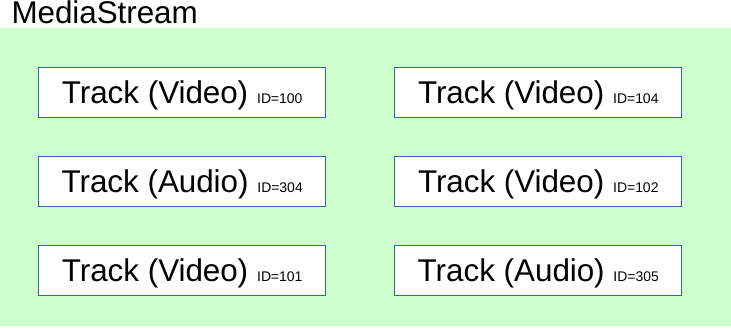
\includegraphics[width=0.6\textwidth]{\webrtcdir/figures/figuras_utilizadas/MediaStream_boxflow.png}
\par\end{centering}
\caption{\label{fig:webrtc:MediaStream:MediaStream_boxflow} Media Stream object}
\end{figure}

The two main components in the MediaStream API are the MediaStreamTrack and
MediaStream interfaces. MediaStreamTrack object represents media of a single
type that originates from one media source, e.g. video produced by a web cam.
A MediaStream object is used to group several MediaStreamTrack objects into one unit
that can be recorded or rendered in a media element.
Each MediaStream can contain zero or more MediaStreamTrack objects. 

A MediaStream object can be created from many MediaStreamTrack also from 
existing media streams or tracks using the MediaStream() constructor.
The constructor argument can either be an existing MediaStream object
in which case all the tracks of the given stream are added to the new MediaStream
object, or an array of MediaStreamTrack objects.
Figure \ref{fig:webrtc:MediaStream:MediaStream_boxflow} illustrates the composition
of a MediaStream object.

The tracks that compose a MediaStream are stored in a track set. The track set must
contain the MediaStreamTrack objects that correspond to the tracks of the stream.
The order of the tracks inside the set is defined by the User and the API never will put
any requirement on the order.
The way to find a specific MediaStreamTrack inside a MediaStream object is to search by 
its MediaStreamTrack ID.

%--------------------------------MediastreamTrack--------------------------------------------------------------------------------- 
A MediaStreamTrack can be in two states in its life-cycle: live or ended.
In the live state mode the track is available for being used.
A live track can be active or muted (disabled).
A muted MediaStreamTrack renders either silence (Audio) 
or black frames (Video), or zero information in general.
Normally a Streamed is muted when the source is temporally unable to provide the track
with data. A track can be muted by the end user.
In the ended state mode the track is disabled because the source is disconnected or disabled.

All tracks in a MediaStream are intended to be synchronized when rendered but different 
MediaStream objects do not need to be synchronized.
While the intent is to synchronize tracks, it could be better in some
circumstances to permit tracks to lose synchronization. In particular,
when tracks are remotely sourced and real-time, it can 
be better to allow loss of synchronization than to accumulate delays 
or risk glitches and other artifacts. Implementations are expected to 
understand the implications of choices regarding synchronization of
playback and the effect that these have on user perception.

Next we show in some tables the main attributes and methods of MediaStream
and MediaStreamTrack.


\begin{table}[!ht]
\caption{MediaStream Attributes}
\label{tbl:MediaStream Attributes}
\centering
\begin{footnotesize}
\begin{tabular}{l l}
\hline
\texttt{active} & Return true if MediaStream is active and false otherwise \\
\texttt{ID} & Identifier string ``UUID 36 characters long''\\
\texttt{onaddtrack} & The event type of this event handler is addtrack\\
\texttt{onremovetrack} & The event type of this event handler is removetrack\\
\hline 
\end{tabular}
\end{footnotesize}
\end{table} 



\begin{table}[!ht]
\caption{MediaStream methods}
\label{tbl:MediaStream methods}
\centering
\begin{footnotesize}
\begin{tabular}{l l}
\hline
\texttt{addtrack} & Adds the given MediaStreamTrack to this MediaStream\\
\texttt{clone} & Clones the given MediaStream and all its tracks\\
\texttt{getAudioTracks} & Returns a sequence of MediaStreamTrack objects representing the AudioTracks in this stream\\
\texttt{getTrackById} & Returns a MediaStreamTrack object from this stream track set whose id is equal to trakId\\
\texttt{getTracks} & Returns a sequence of MediaStreamTrack objects representing all the tracks in this stream\\
\texttt{getVideoTracks} & Returns a sequence of MediaStreamTrack objects representing the VideoTracks in this stream\\
\texttt{removeTrack} & Removes the given MediaStreamTrack object from this MediaStream\\
\hline 
\end{tabular}
\end{footnotesize}
\end{table} 

\begin{table}[!ht]
\caption{MediaStreamTrack Attributes}
\label{tbl:MediaStreamTrack Attributes}
\centering
\begin{footnotesize}
% con p{12cm} se hace una columna de 10cms.
\begin{tabular}{l p{10cm}}
\hline
\texttt{enabled} & The enabled attribute controls the enabled state for the object. \\
\texttt{ID} & ID attribute MUST return the value to which it was initialized when the object was created.\\
\texttt{kind} & The kind attribute MUST return the string "audio" if this object represents an audio track or 
"video" if this object represents a video track.\\
\texttt{label} & The label attribute MUST return the label of the object's corresponding source, if any.\\
\texttt{muted} & The muted attribute MUST return true if the track is muted, and false otherwise.\\
\texttt{onended} & The event type of this event handler is ended.\\
\texttt{onmute} & The event type of this event handler is mute.\\
\texttt{onoverconstrained} & The event type of this event handler is overconstrained.\\
\texttt{onunmute} & The event type of this event handler is unmute.\\
\texttt{readyState} & The readyState attribute represents the state of the track. It MUST return the value as most recently set by the User Agent.\\
\hline 
\end{tabular}
\end{footnotesize}
\end{table} 
\begin{table}[!ht]
\caption{MediaStreamTrack methods}
\label{tbl:MediaStreamTrack methods}
\centering
\begin{footnotesize}
\begin{tabular}{l p{10cm}}
\hline
\texttt{applyConstraints} & Optional parameter in order to add a new constraint structure to apply to this object\\
\texttt{clone} & Clones this MediaStreamTrack.\\
\texttt{getCapabilities} & The getCapabilities() method returns the dictionary of the names of the constrainable properties that the object supports.\\
\texttt{getConstraints} & The getConstraints method returns the Constraints 
that were the argument to the most recent successful call of applyConstraints(), 
maintaining the order in which they were specified.\\
\texttt{getSettings} & The getSettings() method returns the current settings of all the constrainable 
properties of the object, whether they are platform defaults or have been set by applyConstraints().\\
\texttt{stop} & Set track's readyState attribute to ended.\\
\hline 
\end{tabular}
\end{footnotesize}
\end{table} 

\clearpage
%------------------------------------RTCPeerConnection-------------------------------------------------
\subsubsection{RTCPeerConnection API \label{sec:webrtc:WebRTC Technology}}
%Introduccion
%FIXME GERARD
The RTCPeerConnection interface represents a WebRTC connection between the
local computer and a remote peer. It provides methods to connect to a remote peer,
maintain and monitor the connection, and close the connection once it's no longer
needed.
RTCPeerConnection API doesn't handle the signaling process this means that the user is completely 
free to choose any method.
Communications are coordinated via a signaling channel which is provided by
unspecified means, but generally it is a script in the HTML page at the server using Web Sockets.

The main functionality of this application is to transmit the acquired flow by
the getUserMedia API (Audio, video, Constraints...) and send it to the other peer
managing all the parameters necessary to carry out transmission of multimedia data 
stream, in a simple and transparent way, simplifying all the necessary processes shown 
below.
RTCPeerConnection Handles:
\begin{compactitem}
\item Signal processing and voice engine to remove noise from audio and video data 
and provide echo cancellation.
\item Codec handling and video engine.
\item Compression and decompression of audio and video.
\item Transport and Peer to peer communication in order to find the optimal route through firewalls, 
NATs and relays.
\item Security, encrypting the data to guarantee secure communications.
\item Bandwidth management. 
\end{compactitem}

RTCPeerConnection API only has to send and receive MediaStreamTracks over a peer-to-peer connection.
The encoding of MediaStreamTracks is managed through objects called RTCRtpSenders in the same way, the reception
and decoding of MediaStreamTracks is managed through objects called RTCRtpReceivers.

When a MediaStreamTrack is attached to a RTCPeerConnection via the addTrack method, 
a RTCRtpSenders object is created to be associated with this MediaStreamTrack.
On the other hand, RTCRtpReceivers  are created when remote signaling indicates 
that there are new tracks available.
Then, each MediaStreamTrack and its associated RTCRtpReceivers are surfaced 
to the application via the ``ontrack'' event.

Thus, a RTCPeerConnection object contains a set of RTCRtpSenders representing all the tracks to be sent, 
and a set of RTCRtpReceivers representing tracks that are to be received on this RTCPeerConnection object.
All of these sets are initialized to zero when the RTCPeerConnection object is created.
%A continuacion se muestra el proceso completo de RTCP...

In the following code, a couple of RTCPeerConnection objects are created:

\begin{lstlisting}[style=JavaScript]
 pc = new RTCPeerConnection(null); // local
 pc = new RTCPeerconnection(iceServers); // Using google servers for testing
\end{lstlisting}

In the first declaration we use null as configuration parameter. This configuration 
allow us to perform local tests.
The second configuration has the information to find and access Google servers.

A RTCPeerConnection object has an associated ICE agent, signaling state, ICE gathering state, 
and ICE connection state, these are initialized when the object is created.
ICE stands for Interactive Connectivity Establishment , its a techniques used in NAT(network address translator) 
for establishing communication for VOIP, peer-peer, instant-messaging, and other kind of interactive media.
Typically ice candidate provides the information about the ipaddress and port from where the data is going to be exchanged.

The onaddstream method will be called every time that we get a stream from the remote client.
This means that our connection succeeded and this method will attach a remote video 
to the RTCPeerconnection communication.
%Upon getting a remote stream, we attach it to the remote video element.
Next, we have to atThe encoding of MediaStreamTracks is managed by objects called RTCRtpSenders.tach our local stream to the RTCPeerconnection object to send our streams 
to the remote client.
Finally, we have to create an offer which tells the other client how to interact with us once 
the network connection is established.
This offer has to include information such as possible video formats, 
possible audio formats and so on. 
A typical way of expressing this offer is using the Session Description protocol (SDP), 
which is further discussed in Section \ref{sec:webrtc:sdp}.

Once we have an offer, 
we set the local descriptor to it and then, the descriptor is sended to the signaling server
to be sent to the called party.
\begin{lstlisting}[style=JavaScript]
pc.onaddstream = gotRemoteStream;
pc.addStream(localStream);
pc.createOffer(gotOffer);

function gotOffer(desc) {
pc.setLocalDescription(desc);
sendOffer(desc);}

function gotAnswer (desc) {
pc.setRemoteDescription(desc);
}

function gotRemoteStream(e) {
attachMediaStream(remoteVideo, e.stream);
}
\end{lstlisting}
On the called party, the answering client determine if the received message is a description or an ICE candidate.
If is a description, the answering client will set it as the remote description on his RTCPeerconnection object and
create the answer. After all this work, the application is ready to let the browser directly connect to the called party.
If the message is an ICE candidate, the candidate should be added to the RTCPeerconnection object. The browser will continue
trying candidates until a connection is made or it runs out of candidates.

\subsubsection{RTCDataChannel API} 

Currently sending information is present in many areas like communications, file transfer and video games.
This requires fast communications, low-latency and guaranteeing the security of the data.
The improvements related to audio and video introduced in communications by WebRTC provide a great number of 
advantages listed above, this technology also offers an sending data aimed application in order to send data
directly from one browser to another. In this way we avoid the use of servers and intermediate relays that increase
the latency of the system and the cost of service.
Currently there are other data channels as Websockets, Ajax and many more, but these technologies are designed for client/server
communications.
RTCDataChannel works directly with the RTCPeerConnection API, which allows connectivity between two clients without requiring intermediate servers,
generating a low-latency communication.
RTCDataChannel is designed to replicate exactly the Websockets technology, this allows the application to support sending strings as well as any of the
binary types of JavaScript such as Blob, ArrayBuffer and ArrayBufferView, especially useful for gaming applications.

This technology allow two working modes:

\begin{compactitem}
\item \textbf{Unreliable mode}: This mode does not guarantee the correct transmission of all the packets because works through UDP protocol, but 
eliminates the overhead so it is a faster mode, especially useful for gaming applications.

\item \textbf{Reliable mode}: This mode guarantee the transmission and order of all the packets because works through TCP protocol, but 
adds overhead in order to handling the control and error flow.
\end{compactitem}

Now is possible to share files directly in a browser to browser mode. Building on top of RTCDatachannel means that the transferred file data 
is encrypted and doesn't touch an application provide serves. This functionality, combined with the possibility of connecting to multiple 
clients for faster sharing, makes WebRTC file sharing a strong candidate for the web, just need to follow the next steps:
\begin {enumerate}
 \item Read a JavaScript file.
 \item Make a peerconnection between clients, using RTCPeerConnection.
 \item Create a data channel between clients, using RTCDatachannel.
\end {enumerate}


There are several points to consider with this method:
Normally a reliable mode will be chooses in order to realize the file transfer, because a unreliable Datachannel will take some design effort
for the ACK/retransmit protocol, it may not be much faster than using reliable transport so reliable and unordered should provide the best of both methods.
Another point to consider is the file size, if it is small can be stored and loaded as simple Blob object,  and send it through a reliable channel. 
For larger files a chunking mechanism is required. File chunks are loaded and sent to another peer with chukId metadata so the peer can recognize them. 
The current recommendation for maximum chunk size is 16KB. 

The following code shows an RTCDatachannel example:

A peerConnection object is needed in order to establish the connection between peers thanks to the signaling mechanisms.
Once the dataChannel is created, the client can use it to send and receive data between peers.
There are several event handlers in order to manage the communications inside the DataChannel, they are explained inside the code.
\begin{lstlisting}[style=JavaScript]
var peerConnection = new RTCPeerConnection();

// Establish your peer connection using your signaling channel here
var dataChannel =
  peerConnection.createDataChannel("STUN SERVERS", dataChannelOptions);

dataChannel.onerror = function (error) { //Manages error handling
  console.log("Data Channel Error:", error);
};

dataChannel.onmessage = function (event) { //Specifies a function to be called when the message event is fired on the channel.
  console.log("Got Data Channel Message:", event.data);
};

dataChannel.onopen = function () { //Manages the channel aperture
  dataChannel.send("Hello World!");
};

dataChannel.onclose = function () {
  console.log("The Data Channel is Closed"); //Manage the channel closure
};
\end{lstlisting}


\clearpage
\section{Security}
\subsection{WebRTC Security}
WebRTC implementations can transfer sensitive content, as video, audio, documents etc.
Ensuring communications security is a fundamental requirement for this type of applications,and
from the earliest developments of this technology was taken into account.

WebRTC is developed over many underlying technologies in order to develop all the components
which enable this technology such as the RTCPeerConnection and RTCDataChannel API.
The following figure show all the underlying technologies used by WebRTC.

\begin{figure}[htb]
\begin{centering}
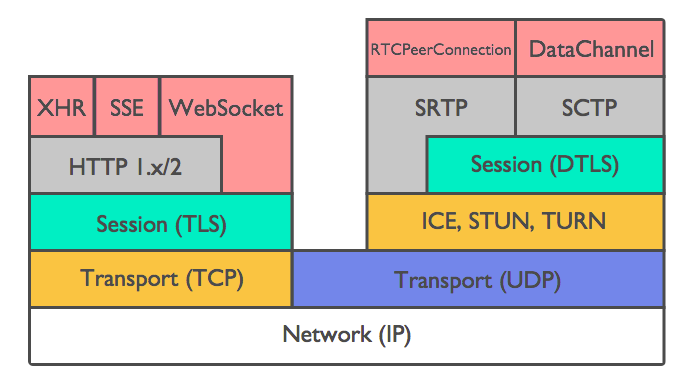
\includegraphics[width=0.7\textwidth]{\webrtcdir/figures/figuras_ok/underlying_tech.png}
\par\end{centering}
\caption{\label{fig:webrtc:WebRTC_security:underlying_tech.png}underlying technologies}
\end{figure}

Many of this technologies have been explained in previous sections such as SDR, STUN, ICE...
The WebRTC architecture assumes from a security perspective that network resources exist in a 
hierarchy of trust. From the user's perspective, the browser or user client is basis of all WebRTC
security, and acts their Trusted Computer Base (TCB).

The browser's job is to enable access to the Internet, while providing adequate security protections to the user. 
The security requirements of WebRTC are built directly upon this requirement; the browser is the portal through which 
the user accesses all WebRTC applications and content.
While HTML and JavaScript provided by the server can cause the browser to execute a variety of actions, the browser segregates 
those scripts into sandboxes. Said sandboxes isolate scripts from each other, and from the user's computer. Generally 
speaking, scripts are only allowed to interact with resources from the same domain - or more specifically, the same "origin".
The browser enforces all security policies that the user desires and is the first step in the verification of all third parties.
All authenticated entities have their identity checked by the browser.

If the user chooses a suitable browser which they know can trust, then all WebRTC communication can be considered "secure" and to follow
the standard accepted security architecture of WebRTC technology. However, if there is any doubt that a browser is 
"trust able" (e.g. having been downloaded from a third party rather than a trusted location), then all following interaction with 
WebRTC applications is impacted and may not be reliably secure.

In other words, the level of trust provided to the user by WebRTC is directly influenced by the user's trust in the browser.

WebRTC is not a plugin, all the underlying technology is installed simply as part of downloading a suitable WebRTC-compatible
browser, such as Chrome or Firefox. As such there is o risk of installation of malware or viruses through the use of an good
WebRTC application. However, WebRTC applications should still be acceded via a HTTPS website signed by a valid authenticator.

Using WebRTC, the browser can access local resources. WebRTC combat this by requiring the user to give explicit permission for the camera
or microphone to be used.
Furthermore, when either the microphone or camera is being used the client UI is required to expressly show the user that the microphone 
or camera are being operated. In Chrome, this takes the form of a red dot on any tab accessing a user's media.

\subsection {HTTPS}
HTTPS (Hypertext transfer protocol secure) is a communication protocol that uses the HTTP (Hypertext transfer protocol secure) and the SSL/TLS
(Secure sockets layer/Transport layer security) protocols to provide encrypted communication and secure identification of a Web Server.
This technology consist of communication over HTTP within a connection encrypted by transport layer security or secure sockets layer.
It creates a secure channel over an insecure network. This ensures reasonable protection from eavesdroppers and man-in-the-middle attacks,
provided that adequate cipher suites are used and that the server certificate is verified and trusted.


HTTP operates at the highest layer of the TCP/IP model, the Application layer; as does the TLS security protocol (operating as a lower sublayer 
of the same layer), which encrypts an HTTP message prior to transmission and decrypts a message upon arrival. Strictly speaking, HTTPS is not 
a separate protocol, but refers to use of ordinary HTTP over an encrypted SSL/TLS connection.

This technology has important security related elements: 

\begin{compactitem}
\item \textbf{Web server authentication}:
The browser ensures the identity of the Web server by validation the server's certificate against the certificate 
of the CA (Certificate authority).
\item \textbf{Communication privacy}:
The browser uses the public key included in the server's certificate to encrypt a secret key to server.
All data exchanged between the server and the browser will be encrypted with the secret key.
\end{compactitem}


\clearpage
\subsection {HTTPS Communication Data Encryption}

Encryption makes impossible for an eavesdropper to determine the contents of communication streams, only parties with access to the secret encryption
key can decode the communication streams.

Encryption is a mandatory feature of WebRTC, and is enforced on all components, including signaling mechanisms. 
Resultantly, all media streams sent over WebRTC are securely encrypted, enacted through standardized and well-known
encryption protocols. 
The encryption protocol used depends on the channel type; data streams are encrypted using Datagram Transport Layer Security (DTLS) 
and media streams are encrypted using Secure Real-time Transport Protocol (SRTP).

\subsubsection{DTLS} 

DTLS (Datagram Transport Layer Security) is a standardized protocol, built into all browsers that support WebRTC, and used in
email and voip communications to encrypt information.
DTLS itself is modeled upon the stream-oriented TLS, a protocol which offers full encryption with \textbf{asymmetric} cryptography methods,
data authentication and message authentication. 


Asymmetric encrypting

\begin{figure}[htb]
\begin{centering}
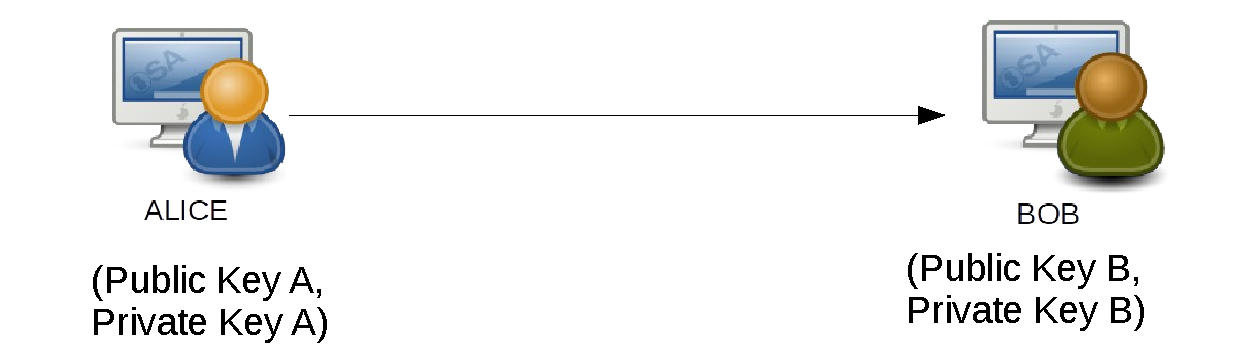
\includegraphics[width=0.7\textwidth]{\webrtcdir/figures/figuras_ok/5_security_assymetric.pdf}
\par\end{centering}
\caption{\label{fig:webrtc:WebRTC_security:5_security_assymetric}Asymmetric encrypting}
\end{figure}

Asymmetric cryptography is a encrypting system that uses two keys, a public key known to everyone and a private or secret key
known only by the recipient of the message.
When Alice wants to send a secure message to Bob, she uses Bob's public key to encrypt the message. Bob then
uses her private key to decrypting.

If Alice wants to send a message to Bob, she must know the public key of Bob, in order to encrypt the message.

$$E(message,Pulickeybob) =encrypted message$$

In the above example, a private message $encrypted message$ is generated using the public key of Bob, $PublickeyBob$, and the message $m$
through an encryption algorithm.

An important element to the public key system is that the public and private keys are related in such a way that only the public key 
can be used to encrypt messages and only the corresponding private key can be used to decrypt them. Moreover, it is virtually impossible 
to deduce the private key if you know the public key.

$$E^{-1}(encrypted message, PrivatekeyBob) = message$$

Public and private key are related, and are the only way to decrypt the initial message.
The decoding algorithm is able to perform the reverse process.

\begin{figure}[h]
\begin{centering}
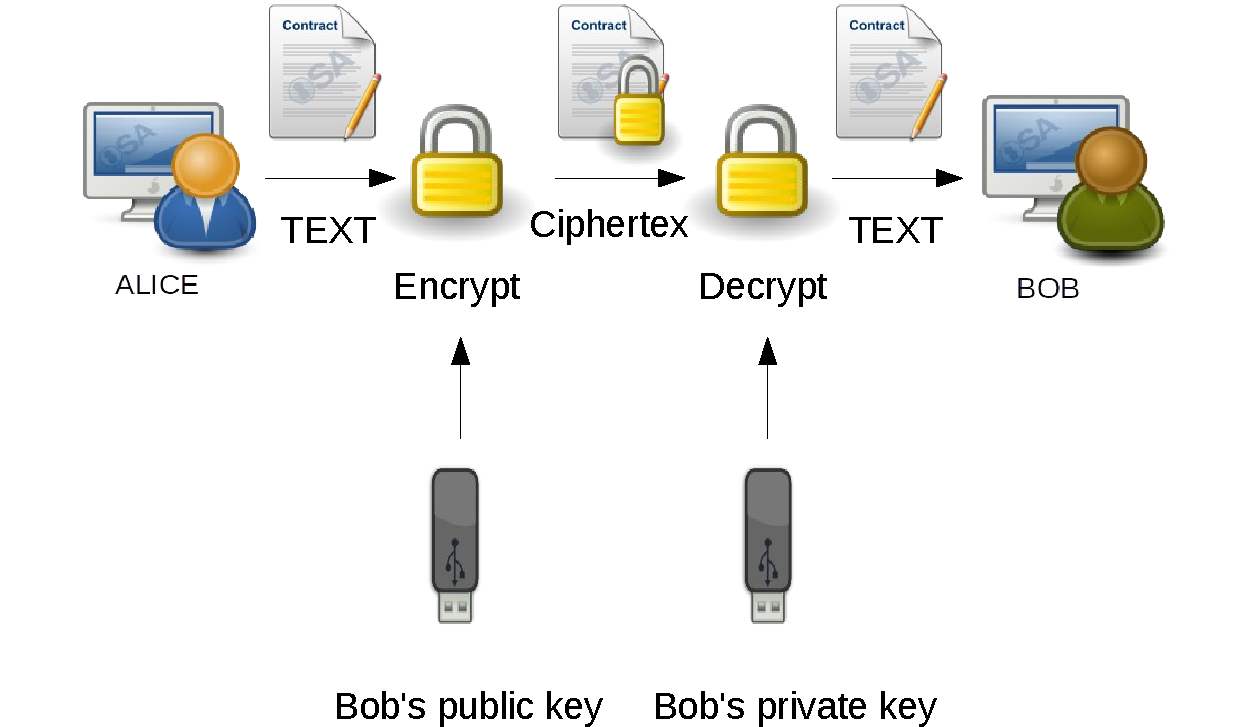
\includegraphics[width=0.7\textwidth]{\webrtcdir/figures/figuras_ok/5_security_Assymetric_full.pdf}
\par\end{centering}
\caption{\label{fig:webrtc:WebRTC_security:5_security_assymetric_full}Assymetric encrypting process}
\end{figure}
This is one of the securest encrypting methods, but slower than others, for this reason WebRTC uses DTLS to encrypt data
because it is more sensitive than other type of media.
\clearpage
\subsubsection {SRTP}
Basic RTP does not have any built-in security mechanisms, and thus places no protections of the confidentiality of transmitted data. 
External mechanisms are instead relied on to provide encryption. In fact, the use of unencrypted RTP is explicitly forbidden by the WebRTC specification.
WebRTC use SRTP for the encryption for mediaStreams because is a lighter-weight option than DTLS.
For encryption and decryption of the data flow, SRTP uses AES as the default cipher. AES is a symmetric-key algorithm, 
meaning the same key is used for both encrypting and decrypting the data.

Symmetric encrypting

The symmetric setting considers two parties who share a key and will use this key to imbue communicated data with various security attributes. 
The main security goals are privacy and authenticity of the communicated data.

Symmetric cryptography is a encrypting system that uses one keys, a secret key known only by the recipient of the message and the sender.
For example, Alice wants to send a message to Bob, first of all, Alice and Bob needs to exchange the key in order to encrypt the message or data.
When both have the key, Alice proceeds to encrypt the message with the key.

\begin{figure}[htb]
\begin{centering}
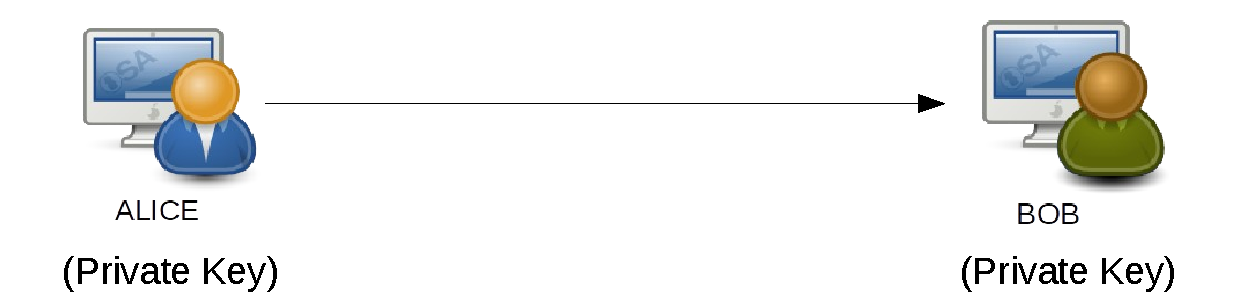
\includegraphics[width=0.7\textwidth]{\webrtcdir/figures/figuras_ok/5_security_symmetric_easy.pdf}
\par\end{centering}
\caption{\label{fig:webrtc:WebRTC_security:5_security_assymetric}Symmetric encrypting}
\end{figure}

When both have the private key, Alice encrypt the message with the key and get the the message encrypted (cipher text C).
$$E(Message,PrivateKey)= Encrypted message$$
Next to that, Alice send the cipher text and bob has to decrypt the received message, passing the private key through a decrypting algorithm.

\begin{figure}[htb]
\begin{centering}
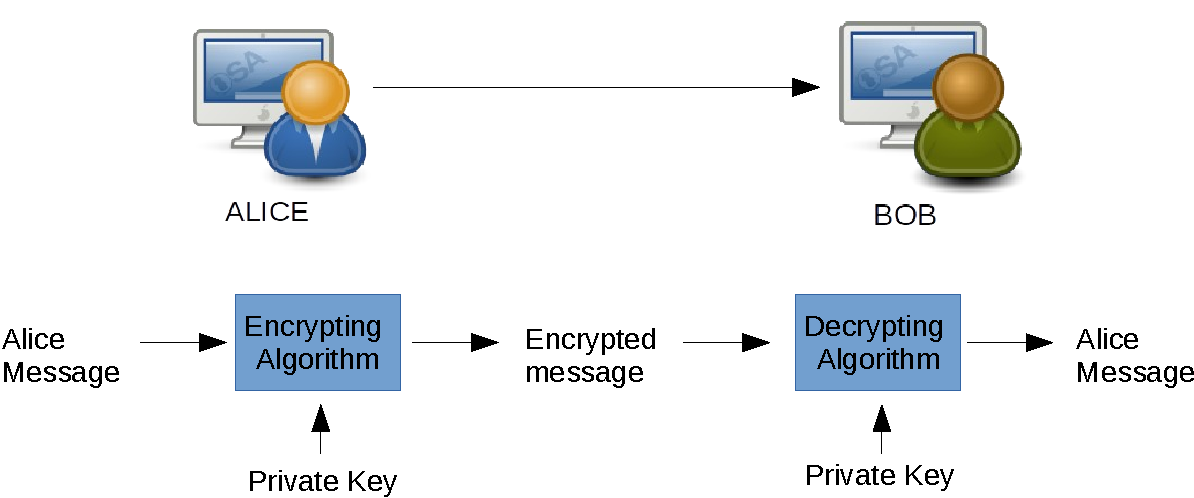
\includegraphics[width=0.7\textwidth]{\webrtcdir/figures/figuras_ok/5_security_symmetric_full_final.pdf}
\par\end{centering}
\caption{\label{fig:webrtc:WebRTC_security:5_security_assymetric}Symmetric encrypting}
\end{figure}

Finally Bob obtains the initial message, with the guarantee that no one else has been able to get the information.
$$E^{-1}(Encrypted message, PrivatekeY) = Message$$

\clearpage
\section{WebRTC Project Implementation}
\subsection{Application Architecture}
The application follows the basic outline for a WebRTC implementation\cite{book1}.
From a general point of view, the following figure illustrates all the devices and components involved in the process and their 
communication mechanism:

\begin{figure}[htb]
\begin{centering}
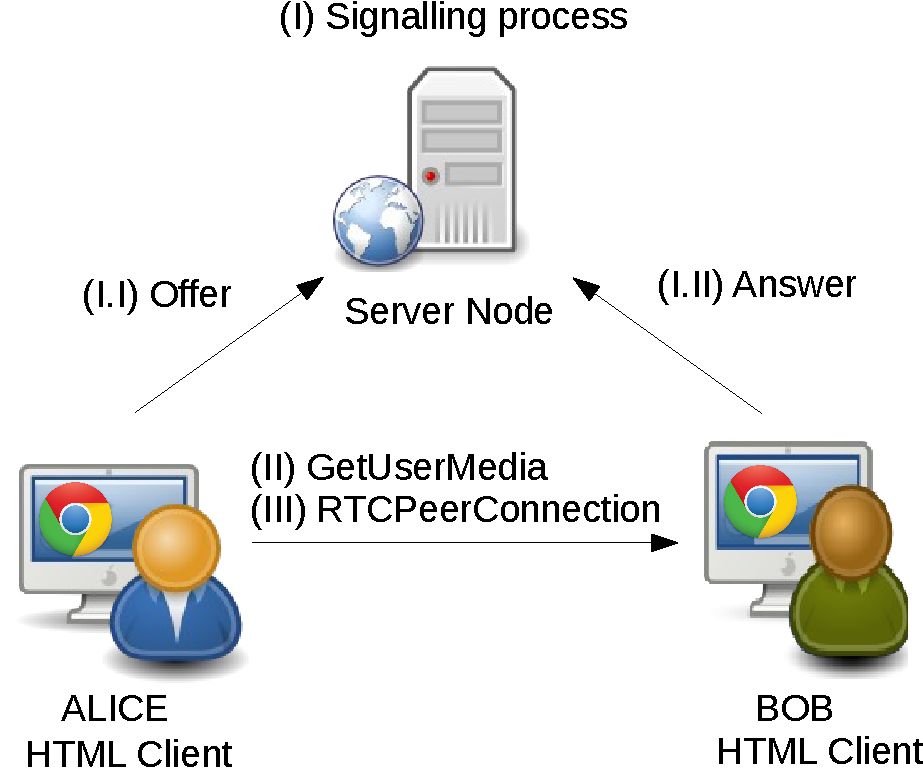
\includegraphics[width=0.5\textwidth]{\webrtcdir/figures/figuras_ok/6_WebRTC_Architecture.pdf}
\par\end{centering}
\caption{\label{fig:webrtc:WebRTC_Architecture:6_WebRTC_Architecture}WebRTC Architecture}
\end{figure}

The architecture can be separated in two parts, server architecture and client architecture, both work separately but are strongly related.

Client Architecture Overview:

The client architecture is very simple, just need a WebRTC compatible browser as the following:

\begin{compactitem}
\item Chrome Browser\cite{Chrome} version 51.0 or later.
\item Firefox Browser\cite{Mozilla} version 45 or later.
\end{compactitem}

Server Architecture Overview:

This side is the responsible for carrying out the signaling process and connect the client side's in order
to establish communication.

Our server is running in a Linux machine by the telematic department by UPC with the following characteristics:
\begin{compactitem}
\item Distribution: Linux
\item Server IP: 147.83.39.232 
\item Ports: 8101 (HTTP), 8102 (HTTPS)
\end{compactitem}
\clearpage

\subsection{Setting Up Server}
In the following code all the modules needed are imported using the require() method.
\begin{lstlisting}[style=JavaScript]
//Getting the modules
var https = require('https');
var fs = require('fs');
var path = require('path');
var express = require('express.io'); 
\end{lstlisting}
In order to enable the server to handle HTTPS connections, the server need to read the keys and certificates
created through OPENSSL in Linux.
\begin{lstlisting}
$ openssl genrsa 1024 > file.pem //Generating RSA KEY.
$ openssl req -new -key file.pem -out csr.pem 
//Input data in order to generate crs.pem
$ openssl x509 -req -days 365 -in csr.pem -signkey file.pem -out file.crt 
//SSL certificate saved
\end{lstlisting}

\begin{lstlisting}[style=JavaScript]
  //Key & Certificate for https server.
  var options = {
	key:fs.readFileSync('./cert/file.pem'),
	cert:fs.readFileSync('./cert/file.crt')
  };
\end{lstlisting}
HTTPS server creation, request and response.
\begin{lstlisting}[style=JavaScript]
app.https(options).io();
var PORT = 8102; //Defined HTTPS server port
//var PORT = 8101; //Defined HTTP server port
console.log('server started and listen to port: ' + PORT);
//ask for static files on the public directory
app.use(express.static(__dirname + '/public'));

app.get('/', function(req, res){ //When a request comes index.ejs is provide to the client
    res.render('index.ejs');
});
\end{lstlisting}
Every time that a client connect/disconnect to the server a message on the console of the server
will be printed.
\begin{lstlisting}[style=JavaScript]
//Display on the console connected/disconnected users
app.io.on('connection' , function(socket){
	console.log("A user connected!!");
	socket.on('disconnect', function() {
        // make your disconnection actions
        console.log("User disconnected!!");
	})
})
\end{lstlisting}
\clearpage
Announcement of a client connection and joining into the room introduced by the user at the beginning of the connection.
The room and the signal room have to be the same

\begin{lstlisting}[style=JavaScript]
//message other clients when some new user enter to the chatroom
app.io.route('ready', function(req){
    //req.data bring the name of the room (for textchat and signaling room)
    req.io.join(req.data.chat_room);
    req.io.join(req.data.signal_room);
    req.io.join(req.data.files_room);
    //Send a broadcast message to the room with name req.data
    app.io.room(req.data).broadcast('announce', {
        message:'New client in the ' + req.data + 'room.'
    });    
})
\end{lstlisting}
This function set up the listening port able to receive connections:
\begin{lstlisting}[style=JavaScript]
app.listen(PORT);
\end{lstlisting}

\subsubsection{Signaling Channel}
This is really similar to the implementation of text chat messages.
One key difference with the text chat is that the sender will not receive his own message
because of using req() method instead off app.io.room.
\begin{lstlisting}[style=JavaScript]
//Signaling process
app.io.route('signal', function(req){
    req.io.room(req.data.room).broadcast('signaling_message', {
        type:req.data.type, 
        message:req.data.message
    });
})
\end{lstlisting}
\begin{lstlisting}[style=JavaScript]
 
\end{lstlisting}

\subsubsection{Text chat}
This function sends a broadcast message to all the clients (sender included), that are connected in to the same room.
\begin{lstlisting}[style=JavaScript]
//Sending text messages to the connected clients 
app.io.route('send', function(req){
    app.io.room(req.data.room).broadcast('message', {
        message:req.data.message,
        author:req.data.author
    });
   
})
\end{lstlisting}
Some functions will be added on the client side in order to send messages to the server, and realize the communication.
\clearpage
\subsection{Setting Up Client}
The following code illustrate all the variable definitions in order to link the HTML tags with
the JavaScript variables and to perform the configuration of the room and iceServers.
\begin{lstlisting}[style=JavaScript]
//Referencing to video tags
var myVideoArea = document.querySelector("#myVideoTag");
var theirVideoArea = document.querySelector("#theirVideoTag");
//Reference to the video selector
var videoSelect = document.querySelector('#camera');
//Referencing to chat text selector
var myName = document.querySelector("#myName");
var myMessage = document.querySelector("#myMessage");
var sendMessage = document.querySelector("#sendMessage");
var chatArea = document.querySelector("#chatArea");
var clear = document.querySelector("#clear");
var ROOM = prompt('type a room name');

var SIGNAL_ROOM = ROOM;
var FILES_ROOM = "files";
//Referencing to signaling messages
  var signalingArea = document.querySelector("#signalingArea");

var configuration = {
'iceServers': [{
  'url': 'stun:stun.l.google.com:19302',
  'url': 'stun:stun1.l.google.com:19302'
}]
};
var rtcPeerConn;
};
           
\end{lstlisting}
\subsubsection{Media Devices}
In WebRTC getUserMedia is not implemented in the same way for all the browsers, the next code try to several different calls
and at least one of them will return a valid reference.
If any of this three calls to getUserMedia works, the navigator will contain a valid reference.
\begin{lstlisting}[style=JavaScript]
if (typeof MediaStreamTrack === 'undefined' || typeof MediaStreamTrack.getSources === 'undefined') {
  document.querySelector("#cameraSelector").style.visibility = "hidden";
} else {
  MediaStreamTrack.getSources(getCameras);

}
\end{lstlisting}
This method find all the media devices connected to the computer by the video type, such as web cams.
It is used if the client has more than one video input device.
\begin{lstlisting}[style=JavaScript]
function getCameras(sourceInfos) {
      for (var i = 0; i < sourceInfos.length; ++i) {
	  var sourceInfo = sourceInfos[i];
	  var option = document.createElement('option');
	  option.value = sourceInfo.id;
	  if (sourceInfo.kind === 'video') {
	  option.text = sourceInfo.label || 'camera' + (videoSelect.length + 1);
	  videoSelect.appendChild(option);
	  }
      }
  }
\end{lstlisting}
\subsubsection{Setting Up the Socket.io Client}
Connecting the socket client to the socket server.
\begin{lstlisting}[style=JavaScript]

//Connect to our socket server
io = io.connect();
//Message type 'ready' implies that our server will announce a new client join to the room.
io.emit('ready', {
    "chat_room": ROOM,
    "signal_room": SIGNAL_ROOM,
    "files_room":FILES_ROOM
});

//Handling the announcement: Display when new user has join into the room
io.on('announce', function (data) {
    displayMessage(data.message);
});
\end{lstlisting}
This functions allow to exchange text messages in both directions client/server.
\begin{lstlisting}[style=JavaScript]
//Handling the text message
io.on('message', function (data) {
    displayMessage(data.author + ": " + data.message);
});

//Listener for "submit button". When "submit" is pressed, socket "emit" a json object to the server.
    sendMessage.addEventListener('click', function (ev) {
  io.emit('send', {
	    "author": myName.value,
	    "message": myMessage.value,
	    "room": ROOM
	});
	ev.preventDefault();
    }, false);	
           
\end{lstlisting}
\subsubsection{Client Signaling Process}
Io.emit () function sends the first signaling message to any client listening.
\begin{lstlisting}[style=JavaScript]
 io.emit('signal', {
                "type": "user_here",
                "message": "Are you ready for a call?",
                "room": SIGNAL_ROOM
            });
\end{lstlisting}
When a server receives a message from a client, it will be shown in the current chat area tag.
\begin{lstlisting}[style=JavaScript]
io.on('signaling_message', function (data) {
      displaySignalMessage("Signal received: " + data.type);
\end{lstlisting}
\clearpage
\subsubsection{Creating The RTCPeerConnection}
Each time the client receives a signaling message from the server, the io.on handler does is to check that if the 
RTCPeerConnection has been initialized, if is not initialized the handler calls the startSignaling() method.
After a RTCPeerConnection has been initialized, the next step is save the message received from the server by a JSON
file in to a variable in order to check the type of the signaling message received.
If it is an SDP message that means the remote party has made and offer. In order to respond this offer the RTCPeerConnection will be invoked
and will create a response by sending the SDP via localDescriptionProtocol method.
If it is not an SDP message, must be an IceCandidate, and the RTCPeerConnection is invoked in order to add this IceCandidate.
\begin{lstlisting}[style=JavaScript]
io.on('signaling_message', function (data) {
    displaySignalMessage("Signal received: " + data.type);
    
//Setting up the RTC Peer Connection object

if (!rtcPeerConn) {
    console.log("Start Signaling?");
    startSignaling();
    
    console.log('Yes, Signalingng has been started!!');
}
if (data.type != "user_here") {
    var message = JSON.parse(data.message);
    if (message.sdp) {
	rtcPeerConn.setRemoteDescription(new RTCSessionDescription(message.sdp), function () {
	    //if we have received an offer, we need to answer
	    if (rtcPeerConn.remoteDescription.type == 'offer') {
		rtcPeerConn.createAnswer(sendLocalDesc, logError);
	    }
	}, logError);
    } else {
	rtcPeerConn.addIceCandidate(new RTCIceCandidate(message.candidate));
    }
}
});
\end{lstlisting}
\clearpage
First of all the function initialize the RTCPeerConnection with the configuration parameters defined above.
Next to that, a different event handler are added in order to receive offers and IceCandidates.
The onnegotiationneeded will be triggered when the Alice receives and SDP offer and Alice will return an answer
to Bob. The SDP offer is generated by sendLocalDesc() method defined below.
The last event handler include in the startSignaling() method is onaddstream(), when this event handler receives a stream from their 
own peer, add this stream to the video area of the another client.
\begin{lstlisting}[style=JavaScript]
            function startSignaling() {
                displaySignalMessage("starting signaling...");
		rtcPeerConn = new RTCPeerConnection(configuration,null);
                //Send any ice candidates to the other peer
                rtcPeerConn.onicecandidate = function (evt) {
                    if (evt.candidate) {
                        io.emit('signal', {
                            "type": "ice candidate",
                            "message": JSON.stringify({
                                'candidate': evt.candidate
                            }),
                            "room": SIGNAL_ROOM
                        });
                        displaySignalMessage("Completed that ICE candidate");
                    }
                };
                //let the 'negotiationneeded' event trigger offer generation (SDP offer)
                rtcPeerConn.onnegotiationneeded = function () {
                    displaySignalMessage("on negotiation called");
                    rtcPeerConn.createOffer(sendLocalDesc, logError);
                };

                //Once remote stream arrives, show it in the remote video element
                rtcPeerConn.onaddstream = function (evt) {
                    displaySignalMessage("going to add their stream...");
                    theirVideoArea.src = URL.createObjectURL(evt.stream);
                };

\end{lstlisting}
\subsubsection{Getting The Media}
Figure below shows a key function in order to get the media from the client computer. This method is called after the signaling process has been completed.
The function receives three parameters, the constraints (in order to turn on the audio and video) and two callbacks methods names one for a success
connection to camera or audio (this one is called if a MediaStream is passed), and one for a failed connection (which is called if an error object is passed).  
This method pertains to startSignaling() function but it is explained here to better understand the process.
\begin{lstlisting}[style=JavaScript]
                //This goes inside startSignaling() function.
                navigator.getUserMedia({
                    'audio': true,
                    'video': true
                    //Once the stream is created, display in myVideo tag, and add our stream as a source of audio/video to our RTCPeerConn    
                }, function (stream) {
                    displaySignalMessage("going to display my stream...");
                    //Adding the local stream to the video tag.
                    myVideoArea.src = URL.createObjectURL(stream);
                    //
                    rtcPeerConn.addStream(stream);
                }, logError);
\end{lstlisting}
This function creates a local session description protocol (SDP) containing information about the video codecs, resolutions, log information, etc.
\begin{lstlisting}[style=JavaScript]
 function sendLocalDesc(desc) {
                rtcPeerConn.setLocalDescription(desc, function () {
                    displaySignalMessage("sending local description");
                    console.log(rtcPeerConn.localDescription);
                    io.emit('signal', {
                        "type": "SDP",
                        "message": JSON.stringify({
                            'sdp': rtcPeerConn.localDescription
                        }),
                        "room": SIGNAL_ROOM
                    });
                }, logError)
            }
\end{lstlisting}
\clearpage

%%\subsection{Passing Data Within DataChannel}
\section{Testing}
This section shows some performance tests in order to ensure the proper system operation.
\begin{enumerate}
\item Establishing connection with the UPC telematics server:
\begin{figure}[htb]
\begin{centering}

\includegraphics[width=1.2\textwidth]{\webrtcdir/figures/webrtcinternals/capturas/1.png}
\par\end{centering}
\caption{\label{fig:webrtc:WebRTC_testing:url}Server}
\end{figure}
\item The caller party chooses the name of the room in order to create the signaling between the clients.
When the called party wants to connect with the caller party, only have to enter the same room name and choose the name
that will be seen.
\begin{figure}[htb]
\begin{centering}
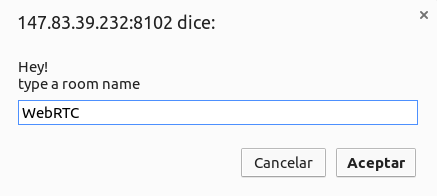
\includegraphics[width=0.7\textwidth]{\webrtcdir/figures/webrtcinternals/capturas/2.png}
\par\end{centering}
\caption{\label{fig:webrtc:WebRTC_testing:room}Room}
\end{figure}
% \begin{figure}[htb]
% \begin{centering}
% 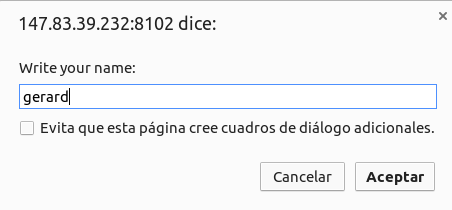
\includegraphics[width=0.7\textwidth]{\webrtcdir/figures/webrtcinternals/capturas/3.png}
% \par\end{centering}
% \caption{\label{fig:webrtc:WebRTC_testing:Name}Name}
% \end{figure}
\item The signaling process start to run until both clients know each other through the processes previously
mentioned.
At the bottom of the page the signaling information is presented.
\begin{lstlisting}
Signaling Messages:

Signal received: SDP
starging signaling...
Signal received: ice candidate
Signal received: ice candidate
Signal received: ice candidate
Signal received: ice candidate
going to add their stream...
sending local description
Completed that ICE candidate
going to display my stream...
on negotiation called
sending local description
Signal received: ice candidate
Signal received: ice candidate
Signal received: ice candidate
Signal received: ice candidate
Signal received: ice candidate
Signal received: ice candidate
Signal received: SDP 
Completed that ICE candidate 
\end{lstlisting}
\item Then, the connection has been established and the application is fully operational.
\begin{figure}[htb]
\begin{centering}
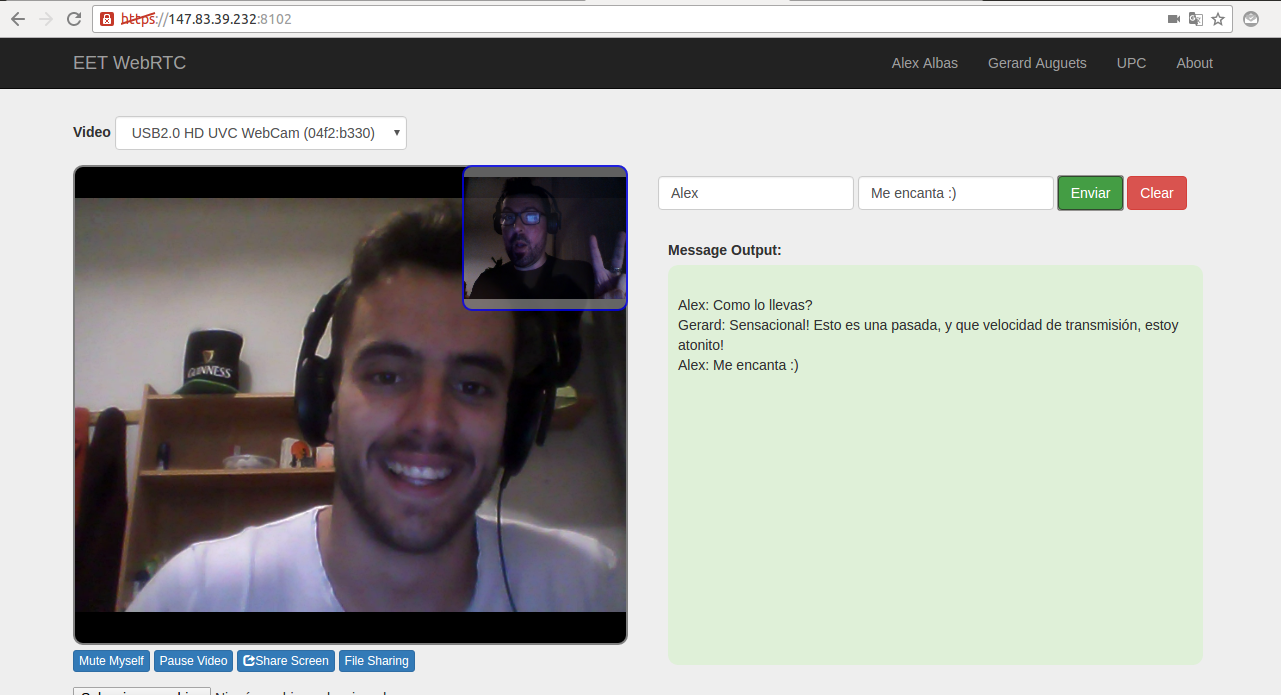
\includegraphics[width=1\textwidth]{\webrtcdir/figures/figuras_ok/App.png}
\par\end{centering}
\caption{\label{fig:webrtc:WebRTC_testing:Name}WebRTCEET}
\end{figure}
\item As observed below the socket.io text-chat server is running
and working.
\begin{figure}[htb]
\begin{centering}
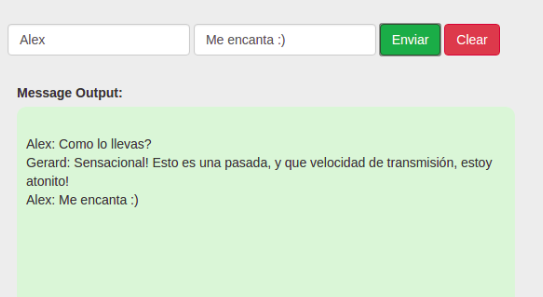
\includegraphics[width=0.7\textwidth]{\webrtcdir/figures/figuras_ok/chat.png}
\par\end{centering}
\caption{\label{fig:webrtc:WebRTC_testing:Name}Text-Chat}
\end{figure}
\end{enumerate}
\clearpage
\subsection{Statistics and graphs}
Another strong point of WebRTC (Only for Chrome) is the possibility to view the multimedia flows
that are running over a communication.
With the tool Webrtc-internals, the MediaStream can be analyzed both you send as you get.

The following figures illustrates the analyzed information relative to the sended
audio sources: 
\begin{compactitem}
\item AudioOutputLevel
\item BitsReceivedPerSecond
\item PacketLost
\item PacketsReceivedPerSecond

\begin{figure}[htb]
\begin{centering}
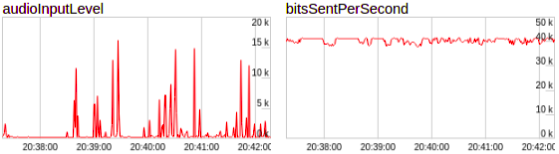
\includegraphics[width=0.9\textwidth]{\webrtcdir/figures/webrtcinternals/1_def.png}
\par\end{centering}
\caption{\label{fig:webrtc:WebRTC_testing:Name}WebRTC internals}
\end{figure}
\begin{figure}[htb]
\begin{centering}
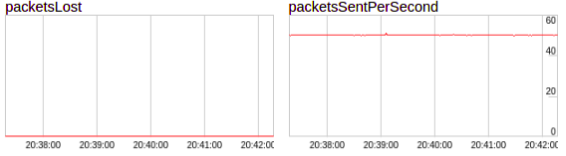
\includegraphics[width=0.9\textwidth]{\webrtcdir/figures/webrtcinternals/1_1_def.png}
\par\end{centering}
\caption{\label{fig:webrtc:WebRTC_testing:Name}WebRTC internals}
\end{figure}

\clearpage
The following figures illustrates the analyzed information relative to the sended
video sources:
\begin{figure}[htb]
\begin{centering}
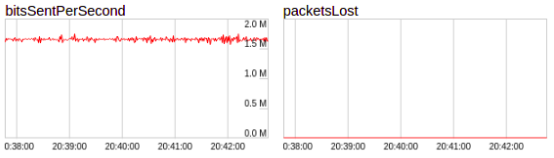
\includegraphics[width=0.9\textwidth]{\webrtcdir/figures/webrtcinternals/video_send_1.png}
\par\end{centering}
\caption{\label{fig:webrtc:WebRTC_testing:Name}WebRTC internals}
\end{figure}
\begin{figure}[htb]
\begin{centering}
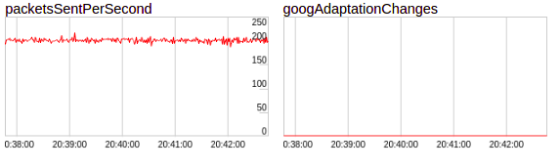
\includegraphics[width=0.9\textwidth]{\webrtcdir/figures/webrtcinternals/video_send_2.png}
\par\end{centering}
\caption{\label{fig:webrtc:WebRTC_testing:Name}WebRTC internals}
\end{figure}
\end{compactitem}

\clearpage

\section{Conclusions}
Finally, we conclude with a very satisfactory rating for the project development and the system implementation.
Following the main guidelines set at the beginnning, the obtained result is very close to the main requirements, achieving good
results in all the project areas, such as the implementation of an application that handles real time multimedia communications through WebRTC
without the use of pluggins using a simple web browser, the implementation of extra functionalities such as text chat, streaming handles, 
room selection, server creation, and of course, without forgetting the learning about the knowledge required in order to carry it out.

This application fits very well in the academic sector, as it was intended, facilitating the communications between the student and teacher.
The functionality is transposable to many fields such as medicine, sale or information business, this place the WebRTC technology
as a strong candidate to overrule the field of the real time communications in a near future.

Technically we have seen the solidity of this new technology, the new possibilities that offer in the real time communications field,
and the efficiency improvements presented against its competitors, improving latency times, the quality of the video and audio, the security 
over the involved systems, increasing the ease and versatility in any computer.
On the other hand, it is a very recent technology, so there are not many examples in order to provide reliability.
In addition, there is a continuous variation in their native functions as well as the browser version, creating some inestability.

From an academic point of view, this project has been a very enriching personal contribution, providing a wealth of knowledge related
to real time communications, the mecanisms and technologies related with WebRTC and their predecessors, many programation languajes and a significant
improvement in the analysis about communication systems.

As a personal conclusion, we finish this project with a great satisfaction, a great ride, and an improved vision about all the 
themes treated in the sections of this project.
We hope to continue in the near future.

\clearpage

\section{Future Implementations}
This project includes the following features:
\begin{compactitem}
\item Video conference
\item Chat
\item Room creation
\end{compactitem}
The programming of this project is a Low-level implementation, avoiding the use of API's developed by third parties, this allows 
the base to be used as a solid starting point for future deployments.

Here is a list of functional improvements that can be easy implemented through the designed system:
\begin{enumerate}
\item Screen Sharing: 
This improvement allows screen sharing between users in a secure way using the implemented WebRTC protocols. 
The transmission will be realized by RTCDataChannel such as video conference.
Screen Sharing is developed in the code of the present project but actually can not be operative because Chrome browser
has disabled this possibility without the use of plug-ins or browser extensions because of the vulnerability caused in their systems.
\item File Transfer: 
Enables sending files in a direct way between two clients without a intermediate server to store the data, as previous features,
sending will be made by RTCDataChannel.
\item Interactive Board:
Interactive board allow both clients to interact with a blackboard to draw. Both clients can observe changes in the board at the same time. 
Very useful for learning environments.
\item Multi conference:
Similar to a simple WebRTC communication, Multi conference allow for communication between multiple clients.
This improvement is useful for five users.
\item Co-browsing: 
Enables to interact with the screen of another client, useful to indicate or modify content.
This improvement suffers the same limitation that Screen Sharing and can not be implemented without plugins because of security problems.
\end{enumerate}

\clearpage

\section{Annexed}
The code is available for all the scientific community in the following repository.
Everybody can download it and try, for own implementation nonprofit.

https://github.com/eetwebrtc/WebRTC




% \section{Practices}
% \input{\dnsdir/practs/inputs}

\ifSOLS
\newpage
\section{Answers to practices}
\shipoutExercise
\vspace{0.5cm}
\shipoutAnswer
\fi

%FIXME BIB: Jose podéis probar diferentes sytles si queréis..
\bibliographystyle{plain}
% \bibliographystyle{ieeetr}
%\bibliographystyle{alpha}
\bibliography{bib/rfc,bib/mybib.bib}

\end{document}
